\documentclass[electronic,oldfontcommands]{kthesis}

%%%%%%%%%%%%%%%%%
%%%% PACKAGES %%%
%%%%%%%%%%%%%%%%%
\usepackage[utf8]{inputenc}
\usepackage[swedish,english]{babel}
\usepackage{csquotes}
\usepackage[inline]{enumitem}
\usepackage{caption}   % to align the table caption to the right/left

% headers
\usepackage{fancyhdr}
\pagestyle{fancy}
\fancyhf{}
\fancyhead[LE,RO]{\thepage}
\fancyhead[RE]{\leftmark}
\fancyhead[LO]{\rightmark}

\usepackage{lscape}
\usepackage{hyperref}  %for references
\usepackage{amsmath,mathrsfs}
\usepackage{amssymb}  % assumes amsmath package installed
\usepackage{epstopdf}
\usepackage{subfig}
\usepackage{epigraph}
% \usepackage{cite}
\usepackage[
  giveninits=false,
  style=ieee,
  sorting=none,
  sortcites,
  hyperref,
  mincitenames=1,
  maxcitenames=2,
  maxbibnames=10,
  minbibnames=1,
  citestyle=numeric-comp, % for [1, 2] instead of [1], [2]
  backend=biber
]{biblatex}
\bibliography{Refs.bib,bibliography/bibliography.bib}

% included papers
\DeclareBibliographyCategory{thesispapers}
\addtocategory{thesispapers}{Olguin:DemoScaling2018}
\addtocategory{thesispapers}{Olguin:EdgeDroid2019}
\addtocategory{thesispapers}{Olguin:ImpactWCA2021}
\addtocategory{thesispapers}{CLEAVE2022}

\usepackage{cleveref}
\usepackage{graphicx}
\usepackage{bm}	%Command \bm{make bold}
\usepackage{algorithm}
\usepackage{algpseudocode}
\usepackage{algpascal}
\usepackage{multicol}
\usepackage[x11names]{xcolor}
\usepackage{lipsum}
\usepackage[printonlyused]{acronym}
\usepackage{booktabs}
\usepackage{graphicx}
\usepackage[binary-units]{siunitx}
\DeclareSIUnit{\belmilliwatt}{Bm}
\DeclareSIUnit{\dBm}{\deci\belmilliwatt}

\usepackage{xcolor}
\usepackage{pagecolor}
\usepackage{tikz}
\usetikzlibrary{tikzmark,calc,decorations.pathreplacing,shapes,arrows.meta,positioning,automata}
\usepackage[export]{adjustbox}
\usepackage{pgf-umlsd}
%% extension for pgf-umlsd v0.5 2009/09/30, which TeXLive comes along
%% source: https://github.com/lyarbean/Tex-stuff

%% \sidelabel{thread}{side}{label}
%% side: left right above below
\newcommand{\sidelabel}[3]{
    \stepcounter{seqlevel}
    \path
    (#1)+(0.1,-\theseqlevel*\unitfactor-0.7*\unitfactor) node (messbeg) {};
    \draw (messbeg) node[#2] {#3};
}

%% mostly used between altblocks
%% \separateline[line style]{from}{to}
\newcommand{\separateline}[3][dotted, color=black, very thick]{
    \stepcounter{seqlevel}
    \path
    (#2)+(.1,-\theseqlevel*\unitfactor-.8*\unitfactor) node (from) {}
    (#3)+(-.1,-\theseqlevel*\unitfactor-.8*\unitfactor) node (to) {};
    \draw[#1] (from) -- (to);
}

%% \begin{altblock}{from}{condition}{to}
%% %%calls here
%% \end{altblock}
\newenvironment{altblock}[3]{
    \stepcounter{seqlevel}
    \path
    (#1)+(.1,-\theseqlevel*\unitfactor-\unitfactor) node (from) {}
    (#3)+(-.1,-\theseqlevel*\unitfactor-\unitfactor) node (to) {};
    \draw (from) node[above right] {[#2]};
}{}

%%
%\newcommand{\postlevel}{\addtocounter{seqlevel}{+1}}

%% \newthread[thread distance]{color fill style}{left}{right}
% \renewcommand{\newthread}[4][1]{
%     \newinst[#1]{#3}{#4}
%     \stepcounter{threadnum}
%     \node[below of=inst\theinstnum,node distance=1em] (thread\thethreadnum) {};
%     \tikzstyle{threadcolor\thethreadnum}=[fill=#2]
%     \tikzstyle{instcolor#3}=[fill=#2]
% }

\newcommand{\Depth}{2}
\newcommand{\Height}{2}
\newcommand{\Width}{2}

\renewcommand{\labelitemi}{\textcolor{IndianRed3}{\bfseries\textbullet}}

% fancy chapters
\usepackage[Sonny]{fncychap}
\ChNameVar{\normalfont\large\rmfamily}
\ChNumVar{\normalfont\rmfamily\bfseries}
\ChTitleVar{\normalfont\rmfamily\huge}

\usepackage{xparse}
\NewDocumentCommand{\thesischapter}{o m m}{%
   \IfNoValueTF{#1}
     {\chapter[#2]{#2\origtitle{#3}}}
     {\chapter[#1]{#2\origtitle{#3}}}%
}
\newcommand\origtitle[1]{\\
  \parbox{\textwidth}{\normalsize\vspace*{2\baselineskip}#1}}


\usepackage{appendix}
\usepackage{hyperref}

\newenvironment{dedication}{\cleardoublepage\null\vspace{\stretch{1}}\begin{flushright}\itshape}{\end{flushright}\vspace{\stretch{2}}\null}

\newcommand{\citeallnames}
{\AtNextCite{\defcounter{maxnames}{99}}\citename}

\makeatletter
\newcommand{\int@suppauthtitle}{%
  \def\ifciteibid{\@secondoftwo}%
  \renewbibmacro*{cite:name}{}%
  \renewbibmacro*{cite:idem}{}%
  \renewbibmacro*{author}{}%
  \renewbibmacro*{editor+others}{}%
  \renewbibmacro*{translator+others}{}%
  \renewbibmacro*{url}{}%
  \renewbibmacro*{in:}{Refereed article published in\\}%
  \renewbibmacro*{title}{}%
  \renewbibmacro*{annotation}{}}

\newcommand{\suppauthtitle}{\AtNextCite{\int@suppauthtitle}}
\makeatother

\definecolor{titlecolor}{HTML}{ECCEF5}

\newcommand{\thesispaper}[2]
{%
\begin{titlingpage*}
\newpagecolor{titlecolor}
\chapter[#1]{\citefield{#2}{title}}

\begin{flushright}
{\citeallnames{#2}{author}}

\vspace{3em}

\suppauthtitle\fullcite{#2}
\end{flushright}

\thispagestyle{empty}
\clearpage%
\hspace{0pt}\vfill%
\noindent\textcopyright~{\citeyear{#2}~\citelist{#2}{publisher}}

\noindent{Layout has been revised for thesis consistency.}

\vfill\hspace{0pt}%
\end{titlingpage*}%
\restorepagecolor%
}


%%%%%%%%%%%%%%%%%%%%%%%%%%%%%%%%%%%%%%%
%%%%%%%%% Document starts here %%%%%%%%
%%%%%%%%%%%%%%%%%%%%%%%%%%%%%%%%%%%%%%%
\begin{document}

%%%%%%%%%%%%%%%%%%%%%%%%%%%%%%%%%%%%%%%%%%
%%%%%% First and second pages %%%%%%%%%%%%
%%%%%%%%%%%%%%%%%%%%%%%%%%%%%%%%%%%%%%%%%%
\title{ Thesis Title }
\subtitle{\textbf{sub-title}}
\author{Manuel {Osvaldo Jesús} {Olguín Muñoz}}
\date{\today}
\thesistype{Doctoral Thesis}
\imprint{Stockholm, Sweden, \the\year{}}
\examen{Teknologie doktorexamen i elektroteknik}
\disputationsdatum{fredagen den 18 januari 2020 klockan 14.00}
\disputationslokal{Sal F3, Lindstedtsvägen 26, Kungliga Tekniska Högskolan, Stockholm}
\publisher{Universitetsservice US AB}
\address{%
	KTH Royal Institute of Technology\\%
	School of Electrical Engineering and Computer Science\\%
	Division of Information Science and Engineering\\%
	SE-10044 Stockholm\\%
	Sweden%
}
\isbn{ISBN 100-}
%\issn{ISSN XXX} % No longer used at KTH
\trita{TRITA-EECS-AVL-2020:4}
\kthlogo{KTHLogo}

% Create title page using info above
\maketitle

\frontmatter % Pages i, ii, iii, iv, v etc.

\chapter[Abstract]{}

%%%%%%%%%%%%%%%%%%%%%%%%%%%%%%%%%%%
%%%%%%%%%%% ABSTRACT %%%%%%%%%%%%%%
%%%%%%%%%%%%%%%%%%%%%%%%%%%%%%%%%%%
\begin{abstract}
\noindent \lipsum[1]

\end{abstract}

\bigskip \bigskip \bigskip \bigskip \bigskip

\setlength{\leftskip}{0.3 cm} \textbf {Keywords:} Lorem, Ipsum, Dolor, Sit, Amet

%%%%%%%%%%%%%%%%%%%%%%%%%%%%%%%%%%%%%%%%
%%%%%%%% SWEDISH ABSTRACT %%%%%%%%%%%%%%
%%%%%%%%%%%%%%%%%%%%%%%%%%%%%%%%%%%%%%%%
\newpage
\selectlanguage{swedish}
\begin{abstract}
\noindent \lipsum[1]
\end{abstract}
\selectlanguage{english}
\nocite{
    olguinmunoz2018demoscaling,
    olguinmunoz2019edgedroid,
    olguinmunoz2021impact,
    olguinmunoz2022cleave,
    olguinmunoz2022ainur,
    olguinmunoz2023realistic
}

\printbibliography[
    heading=bibintoc,
    title={List of Papers},
    category=thesispapers
]
\todo[inline]{Fix titlecase!!}
%%%%%%%%%%%%%%%%%%%%%%%%%%%%%%%%%%%%%%%
%%%%%%%% ACKNOWLEDGMENT %%%%%%%%%%%%%%%
%%%%%%%%%%%%%%%%%%%%%%%%%%%%%%%%%%%%%%%
\chapter{Acknowledgements}
\epigraph{La educación es, tal vez, la forma más alta de buscar a Dios.}{\emph{Gabriela Mistral}}
\glsresetall%

There are many, many people I owe gratitude to for making this dissertation possible.
I would like to begin by thanking my supervisor, Prof. James Gross.
This dissertation would not have been possible without his guidance and motivation during this long process.
His supervision opened doors that I had never imagined would open for me, and his dry German humor has certainly helped cheer me up whenever I was overwhelmed by some deadline.
Above all, I would like to thank James for his patience and understanding whenever I encountered difficulties, and for the flexibility he has afforded me in completing this Ph.D.

I would like to express my deepest gratitude to Prof. Mahadev ``Satya'' Satyanarayanan, for welcoming me repeatedly, over long periods of time, as a visiting researcher at \gls{CMU}.
Likewise, I'm deeply indebted to Prof. Roberta ``Bobby'' Klatzky of \gls{CMU} for the many helpful and insightful discussions, for introducing me to the field of Human-Computer Interaction, and for always greeting me with a warm smile.
Both Satya's and Bobby's tremendous experience and generosity have been invaluable, and their guidance and advice have certainly shaped my work for the better.

I would also like to thank everybody involved with the defense of this thesis.
I am very grateful to Prof. Yu Xiao of Aalto University, for agreeing to act as my dissertation opponent.
My dissertation defense will certainly benefit greatly from her expertise and insights.
I would like to extend my sincere thanks to my grading committe, consisting of Prof. Ana Aguiar (Universidade do Porto), Prof. Per Gunningberg (Uppsala Universitet), and Prof. Klaus Wehrle (\gls{RWTH}), for investing time and effort into reading and grading this dissertation.
Special thanks also go to Prof. Markus Flierl of \pgls{KTH} for advance-reviewing this dissertation, and to Prof. Mats Bengtsson, also of \pgls{KTH}, for agreeing to act as chairperson for the defense.

Moreover, I extend my thanks to my co-authors and colleagues.
To Samie Mostafavi, Vishnu N. Moothedath, and Neelabhro Roy at \pgls{KTH}, for always being willing to engage in interesting discussions, but also for generally being fun to be around.
And to Dr. Jaya Prakash (IMDEA Networks Institute), Dr. Junjue Wang (\gls{CMU}), and Dr. Padmanabhan ``Babu'' Pillai (\gls{CMU}) for enriching my research with their interesting insights.

I am very lucky and grateful that I got to stay at both \pgls{KTH} and \gls{CMU}, and I would like to thank everyone who made these spaces welcoming and engaging.
A big thank you goes out to my colleagues (both current and former) at the division of \gls{ISE} for all those fun lunches at Restaurang Q, Cypern, and SysterOBror over the years, which always helped to break the monotony of the days.
This includes but is not limited to Samie, Vishnu, Neel, Sahar, Antonios, Germán, Boules, Baptiste, Håkan, Pol, Marie, Wendi, and Sebastian.
I would additionally like to extend a special thank you to Dr. Sebastian Schiessl, for ``taking me under his wing'' when I first arrived at \gls{ISE} and acting as a sort of mentor during my first moths.
Likewise, I extend my gratitute to Gerd Fransson, for greeting me with a huge smile every morning the years our offices faced each other and cheering up my days with her wholesome energy.
I also thank Prof. Joakim Jaldén for giving me the opportunity to act as his teaching assistant.
Another big thank you goes out to everyone (current and former) at Satya's group at \gls{CMU}, for always welcoming me with open arms and treating me like one of them whenever I was visiting.
This includes but is not limited to Junjue, Tom, Roger, Shilpa, Jan, Edmond, Jim, Babu, and Zhuo.
I will always remember our Monday morning talks and Friday lunch outings dearly.

Furthermore, I would like to extend my sincere thanks to Prof. Sandra Céspedes, of Universidad de Chile and Concordia University, for her guidance and urging to embark on this journey towards a Ph.D., and for always being willing to offer help and advice.
Likewise, I'd like to thank Prof. Javier Bustos, of Universidad de Chile and NIC Chile Research Labs, for giving me the opportunity many years ago to first get into distributed systems research.
Also, I'd like to extend my gratitude to Prof. José Miguel Piquer, of Universidad de Chile, for taking me as his ``long-distance'' teaching assistant and allowing me to give back to my \emph{alma mater} from across the ocean.
A very special thanks goes out to Prof. Jérémy Barbay of Universidad de Chile and Universidad de Concepción, for being both a mentor and a friend since the day I took his course on Android programming as an undergraduate student.
I am deeply appreciative of the fact that although our interactions these last few years have been sporadic at best, I can always reach out to him for help and advice when I need them.

\medskip

This dissertation would not have been possible without the help and support of my family.
First and foremost, I would like to thank the love of my life and wife~\footnote{\emph{Future-wife} at the time of writing, but \emph{wife} at the time of the defense of this thesis!}, Andresa.
I could not have done this without her companionship and love.
I am eternally grateful for her unconditional support over difficult periods of time and over tremendous distances while we were living apart, and for making every day we spend together amazing.

I am also deeply grateful to my parents, Gabriel and Valeria, for always encouraging my curiosity and my drive to learn and discover.
They have been my rocks, my pillars, since the day I was born, and I am proud to be their son.
A big thank you goes out to my sister, Paola, as well.
Although we sometimes get on each other's nerves, she has always been there for me and supported me, and I could not have asked for a better sister.
Likewise, I extend my deepest gratitude to everyone in my immediate and extended family who have given me support and love over the years, including but not limited to my paternal grandparents, Manuel and María Yolanda, my maternal grandparents, Caupolicán and María Aura, my uncle Mauricio, his wife Marylen, their daughter Amanda, and everybody else.
I would like to make a special mention to my late grandfather, Caupolicán ``Poli'' Muñoz, who always inspired and fanned the flames of academic curiosity in me.
I hope he would have been proud seeing how far I have come.
Another special mention goes to my uncle Manuel, who graciously took me in and gave me a place to stay at the first few months of my Ph.D. studies.

I would also like to thank all of my friends who have made this long, ardous journey more amenable.
I would particularly like to thank everyone I met through Tartan Salsa, including, but not limited to, Andresa, Jennifer, Alyson, Kuai-Kuai, Carmen, Moataz and Nora, Eric, and many others.
They made Pittsburgh feel like home, even before I finally moved there permanently in 2022.
I also want to thank Ann-Charlotte in Stockholm, for always being so kind, so considerate, and so much fun to be around.
Further, I am deeply grateful to my friends in Chile who have remained a source of support, even though we only get to see each other once a year when I visit.
This includes, but is not limited to, Juan Pablo, Fernanda, Diego, Camila, George, Patricio, Kevin, Pablo, and many others.
Yet another special mention goes to Diego's family, who have always treated me as one of their own.

Finally, I would be remiss in not mentioning my pets and animal friends who have provided me with love and warmth during these years.
I thank my dogs, Aros and Skatt, who I sadly had to leave behind in Chile with my sister, but who still greet me with enthusiastically wagging tails whenever I visit.
And I thank my cats, Mochi and Tiramisú, who, although have only been in my life for about a year, have sweetened and made much more bearable the long days and nights I have spent writing this dissertation.

\bigskip

\noindent{}Manuel Olguín Muñoz\\
Pittsburgh, May 2023
%%%%%%%%%%%%%%%%%%%%%%%%%%%%%%%%
%%%%%%%% ACRONYMS %%%%%%%%%%%%%%
%%%%%%%%%%%%%%%%%%%%%%%%%%%%%%%%
\chapter{Acronyms}
\begin{acronym}
    \acro{CPS}{Cyber-Physical System}
    \acro{NCS}{Networked Control System}
    \acroindefinite{NCS}{an}{a}
    \acro{LAN}{Local-Area Network}
    \acro{WLAN}{Wireless Local-Area Network}
    \acro{KPI}{Key Performance Indicator}
    \acro{WPAN}{Wireless Personal Area Network}
    \acro{CSMA/CD}{Carrier-Sense Multiple Access with Collision Detection}
    \acro{CLEAVE}{ControL bEnchmArking serVice on the Edge}
    \acro{OS}{Operating System}
    \acro{UDP}{User Datagram Protocol}
    \acro{TCP}{Transmission Control Protocol}
    \acro{RMS}{Root Mean Square}
    \acro{RTT}{Round-Trip Time}
    \acro{CI}{Confidence Interval}
    \acro{AP}{Access Point}
    \acro{API}{Application Programming Interface}
    \acro{SSF}{Swedish Foundation for Strategic Research}
    \acro{TECoSA}{Trustworthy Edge Computing Systems and Applications}
    \acro{ABC}{Abstract Base Class}
    \acroplural{ABC}[ABCs]{Abstract Base Classes}
    \acro{URL}{Uniform Record Locator}
    \acro{AWS}{Amazon Web Services}
    \acro{EC2}{Elastic Compute 2}
    \acro{AMI}{Amazon Machine Image}
    \acro{SSH}{Secure Shell}
    \acro{IP}{Internet Protocol}
    \acro{VPN}{Virtual Private Network}
    \acro{NAT}{Network Address Translation}
    \acro{NTP}{Network Time Protocol}
    \acroindefinite{NTP}{an}{a}
    \acro{SDR}{Software-Defined Radio}
    \acroindefinite{SDR}{an}{a}
    \acro{VLAN}{Virtual Local-Area Network}
    \acro{APT}{Advaced Packaging Tool}
    \acro{LTE}{Long-Term Evolution}
    \acro{SSID}{Service Set Identifier}
    \acro{EPC}{Evolved Packet Core}
    \acro{UE}{User Equipment}
    \acro{eNodeB}{Evolved Node B}
    \acro{DNS}{Domain Name System}
    \acro{MNIST}{Modified National Institute of Standards and Technology}
    \acro{HTTP}{Hyper-Text Transfer Protocol}
    \acroindefinite{HTTP}{an}{a}
    \acro{YAML}{YAML Ain't Markup Language}
    \acro{O-RAN}{Open Radio Access Network}
    \acro{FOSS}{Free and Open Source Software}
    \acro{COSMOS}{Cloud enhanced Open Software defined MObile wireless testbed for city-Scale deployment}
    \acro{OMF}{ORBIT Management Framework}
    \acro{POWDER}{Platform for Open Wireless Data-driven Experimental Research}
    \acro{COTS}{Commercial Off-The-Shelves}
    \acro{RF}{Radio-Frequency}
    \acro{VM}{Virtual Machine}
    \acro{REST}{REpresentational Sate Transfer}
    \acro{OS}{Operating System}
    \acro{MaaS}{Metal-as-a-Service}
    \acro{OEDL}{\ac{OMF} Experiment Description Language}
    \acro{RSpec}{Resource Specification}
    \acro{LXC}{LinuX Containers}
    \acro{MEC}{Mobile Edge Computing}
    \acro{USRP}{Universal Software Radio Peripheral}
    \acro{OAI}{OpenAirInterface}
    \acro{NR}{New Radio}
    \acro{FPGA}{Field-Programmable Gate Array}
\end{acronym}

\mainmatter % Pages 1, 2, 3...

\tableofcontents*{}
\part{Summary}
\chapter{Introduction}\label{chap:introduction}

\todo[inline]{
    Introduction here. Why do we need this work?
}

\todo[inline]{
    Reorganize EdgeDroid, Cleave, Ainur, together.

    Pull in multi-loop results for EdgeDroid?

    Think about experiments.
}

\section{Summary of the key contributions of this thesis}

This thesis presents three core contributions to the existing body of research in edge computing, as well as a number of secondary ones.
Firstly, we introduce a methodological approach to studying system responsiveness versus resource consumption trade-offs in edge-bound feedback-loop systems such as \gls{WCA} and \gls{NCS}.
This approach is based on the emulation of the client-side workload, while maintaining the \emph{real} server-side process as well as network stack.
We validate this methodology by example, presenting implementations of its application in the context of \gls{WCA} and \acp{NCS}, and introduce a software framework for the orchestration of the edge computing testbeds necessary for its implementation.

Secondly, we present a deeper exploration of this methodology for \gls{WCA} and introduce the first ever model for the end-to-end emulation of human timing behavior in \gls{WCA}.
This model is built from a thorough characterization of these behaviors, the data for which we obtain from a comprehensive human-subject study.

Finally, as an extension and application of our first and second contributions, we explore the implications of our methodology and human user model on the optimization potential of \gls{WCA} deployments.
In particular, we study the sampling and energy consumption behaviors of these systems with and without considering realistic human behavior.
We conclude that significant improvements can be achieved through the use of our human user model.

\subsection{Overview of each included paper}

\cref{paper:olguinmunoz2018demoscaling,paper:olguinmunoz2019edgedroid,paper:olguinmunoz2022cleave,paper:olguinmunoz2022ainur} introduce and discuss this methodology and the necessary tools for its implementation.
\cref{paper:olguinmunoz2018demoscaling} presents a short, high level overview of this methodological approach as applied to \gls{WCA}, making very straightforward assumptions about human behavior in \gls{WCA} applications.
\cref{paper:olguinmunoz2019edgedroid} extends the discussion from \cref{paper:olguinmunoz2018demoscaling}, providing more details on the implementation of the necessary measurement framework and the tooling employed.
This work presents the first empirical results obtained with our methodological approach, providing thus an initial validation of its utility for research.
\cref{paper:olguinmunoz2019edgedroid} also discusses in detail the assumptions that were made about human behavior and reactions.
We assume in these works a human which is impervious to poor system performance, and suffers no annoyance, fatigue, frustration, nausea or other shortcomings of real human users.
The result is a model of a user who responds in a precisely reproducible and deterministic manner to the same system stimulus every time.

\cref{paper:olguinmunoz2022cleave}, on the other hand, presents a discussion on the implementation of this methodology for \acp{NCS}.
As discussed above, these applications are similarly difficult as \gls{WCA} to benchmark (in particular at scale on multi-tenant systems) due to their client-side complexity, but in particular because of their often extreme sensitivity to latency.
\todo[inline]{More argumentation or refer to previous section.}
We apply thus in this work our methodology to \gls{NCS} through the implementation of a tool for the emulation and subsequent deployment of these systems on edge computing infrastructure.
This tool allows us to both emulate the physical components of a relatively simple control system plant and deploy real algorithms for its control.
The software acts as a middleware which abstracts away the network from the development of these workloads, allowing for quick prototyping and deployment.
This work also showcases the scalability and flexibility of our approach, allowing us to deploy scenarios with a large number of loops without the need for domain-specific hardware.

\cref{paper:olguinmunoz2022ainur} presents a tangential contribution.
It introduces the software framework used in \cref{paper:olguinmunoz2023realistic,paper:olguinmunoz2022cleave} for the orchestration of the edge computing testbeds on which the developed tools were deployed.
This framework represents an ancillary contribution, crucial for the research presented in these works.
Without it, the experimental approach described in these works would not have been feasible.

Next, in \cref{paper:olguinmunoz2021impact,paper:olguinmunoz2023realistic} we delve deep into the implementation of our methodology for \gls{WCA}, as well as study its implications for optimization of these systems.
Although the above approach to human behavior in \gls{WCA} discussed represents a useful initial approximation, it is nonetheless not a realistic model of it.
In \cref{paper:olguinmunoz2021impact} we therefore take the first major step towards such a model, presenting a deep characterization of human behavior in these applications.
We develop this characterization through a human subject study with a cohort of \num{40} participants who were asked to interact with an instrumented \gls{WCA} application.
System responsiveness is altered in real-time during each execution of the task, and we record participants' reactions by measuring task- and system-related metrics, as well as biometrics from sensors placed on their bodies.
Participants were also asked to fill out two personality indicator questionnaires, allowing us to later correlate individual personality traits and measured reaction to changes in system responsiveness.

\cref{paper:olguinmunoz2023realistic} then concludes this line of work, building upon the insights and data obtained in \cref{paper:olguinmunoz2021impact} to develop the first ever data-driven model of human timings for \gls{WCA}.
The model is validated against previously obtained results, both through simulated, controlled executions and deployments on a real edge computing testbed.
This work also explores potential implications of this model for \gls{WCA} system optimization potential, particularly in the domains of energy consumption and sampling strategies.

\section{Structure of this thesis}

\todo[inline]{This thesis is structured as follows.}
\chapter{Key contributions and results}\label{chap:contributions}

\section{A methodology for the study of feedback-loop systems in Edge Computing}\label{summary:methodology}

\begin{figure}
    \centering
    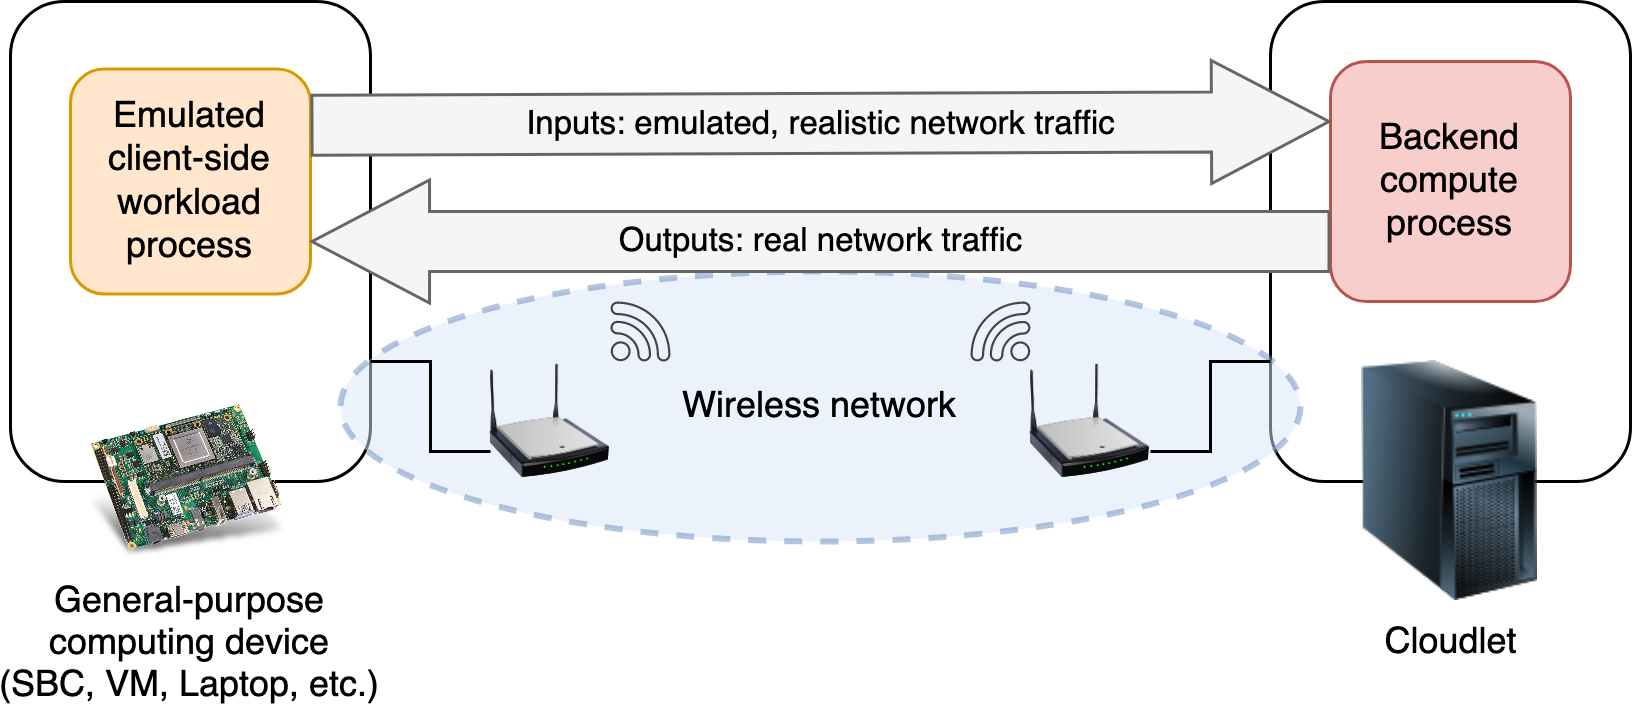
\includegraphics[width=.8\textwidth]{Figs/methodology.png}
    \caption{%
        Overview of the proposed methodology for the study of feedback-loop systems on edge computing infrastructure.
        The  client side of the system is replaced with an emulation executed on a general-purpose computing device.
        The backend/server side of the system along with the network remain unchanged.
    }\label{fig:methodology}
\end{figure}

As discussed above, benchmarking infrastructures for edge-bound applications featuring feedback-loops is challenging, in particular when dealing with applications with high sensitivity to latency (such as \ac{NCS}) or with human involvement (such as \ac{WCA}).
In the following, we introduce our methodological framework for tackling this challenge.

A general overview of our methodology is illustrated in \cref{fig:methodology}.
It is based on the core idea of executing an emulation of the target workload on top of the real hardware on which it is to be deployed.
We replace the client side of the system with a realistic emulation of the desired behaviors; this emulation is implemented in software deployed on \ac{COTS} general-purpose computing devices.
The backend side and the network are not changed.

Two main arguments drive this approach.
One, the difficulty of scaling the number of clients in these systems in a research context.
The systems we target exhibit a centralized nature in which a potentially large number of clients offload computation to a single central compute node.
The client-side component of the applications of interest for this research is often complex to scale, either due to the involvement of humans (as in the case of \ac{WCA}) or due its cyber-physical nature (in \acp{NCS}).
Emulating this component reduces this complexity by moving it into the software domain, allowing for easier scaling through the use of cheap, general-purpose hardware such as single-board computers (e.g. Raspberry Pis, Beaglebones, etc.).

And two, it maintains the realism of the most complex parts of the system.

\todo[inline]{Fix and finish}

In the following, we will discuss the initial implementation of this methodology to two different classes of applications.
We first discuss the methodology in the context of a human-in-the-loop application, \acl{WCA}, in section \cref{ssec:methodology:wca}.
Then, in \cref{ssec:methodology:ncs}, we present an exploration into it's utility for the study of \acf{NCS}.


\subsection{Applying the methodology to \acs{WCA}}\label{ssec:methodology:wca}

\begin{figure}
    \centering
    \begin{subfigure}[b]{.47\textwidth}
        \centering
        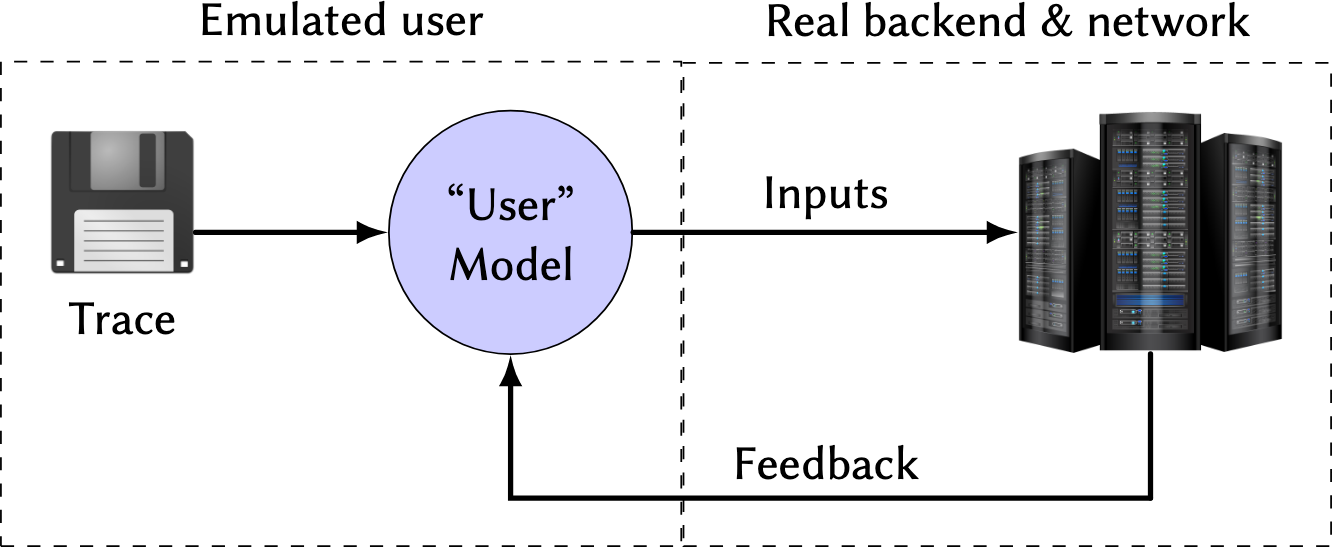
\includegraphics[width=\textwidth]{Figs/trace_edgedroid.png}
        \caption{%
            High level conceptual design of our methodology for \ac{WCA}.
            We replace the human by a trace-driven emulation.
            This allows us to maintain realism in inputs sent over the network to the compute process on the backend, while simplifying the design of the client software.
        }
    \end{subfigure}
    \hfill
    \begin{subfigure}[b]{.47\textwidth}
        \centering
        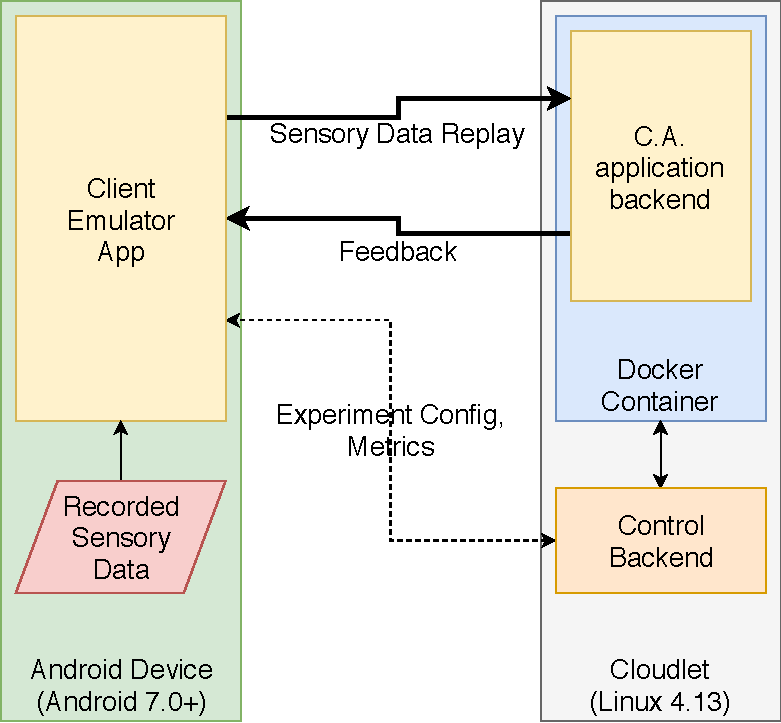
\includegraphics[width=\textwidth]{publications/2018DemoScalingOnTheEdge/img/TraceReplay_GenArch}
        \caption{%
            Architectural overview of the EdgeDroid \num{1.0} tool.
            The ``client emulator app'' implements the aforementioned user model together with the required networking functionality to connect to a \ac{WCA} backend running on a cloudlet.%
            }
    \end{subfigure}\\
    \medskip
    \begin{subfigure}[t]{\textwidth}
        \centering
        \adjustbox{scale=0.7}{
            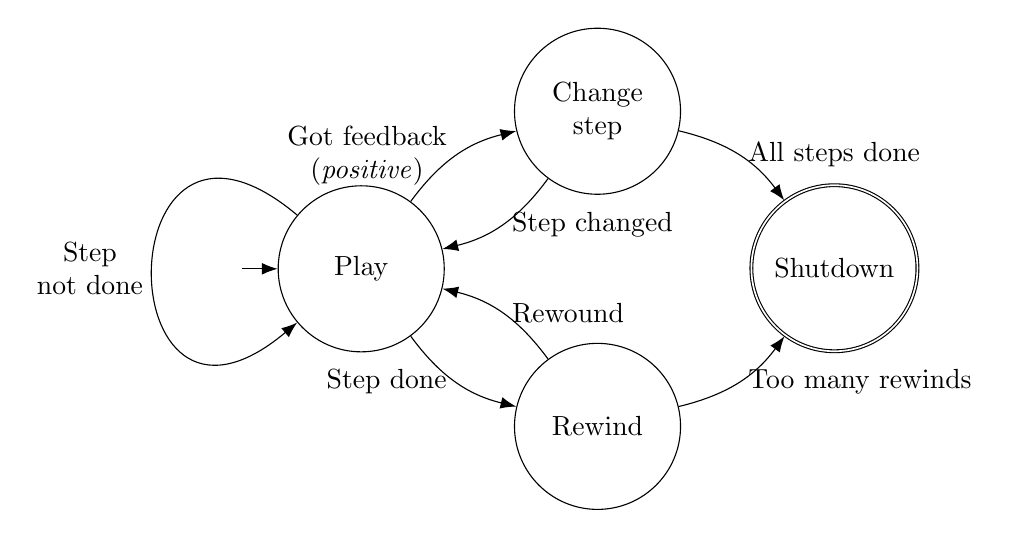
\begin{tikzpicture}[align=center,
            node distance=.5cm and 1.5cm,
            every initial by arrow/.style={-{Latex[length=2mm]}}]
            % Place nodes              
            \node [initial, state, minimum size=6em, initial text=] (play) {Play};               
            \node [state, above right=of play, minimum size=6em] (change) {Change\\step};
            \node [state, below right=of play, minimum size=6em] (rewind) {Rewind};
            \node [state, accepting, above right=of rewind, minimum size=6em] (shutdown) {Shutdown};
            
            % Draw edges
            \path[draw, -{Latex[length=2mm]}]
            (play) edge [bend right=20] node[left] {Step done} (rewind)
            edge [bend left=20] node[left] {Got feedback\\(\emph{positive})} (change)
            edge [out=140,in=220,looseness=6] node[left] {Step\\not done} (play)
            
            (change) edge [bend left=20] node[right] {Step changed} (play)
            edge [bend left=20] node[right] {All steps done} (shutdown)
            
            (rewind) edge [bend right=20] node[right] {Rewound} (play)
            edge [bend right=20] node[right] {Too many rewinds} (shutdown);
            
            \end{tikzpicture}
        }
        \caption{State diagram of the user model governing the replay of the pre-recorded trace at runtime. This model approximates the behavior of an ``ideal'' human, one that is patient and makes no mistakes.}\label{fig:usermodel}
    \end{subfigure}
    \caption{%
        Overview of our first implementation of the methodology for \ac{WCA}.
    }\label{fig:edgedroid1:trace}
\end{figure}

We first introduce our methodology in \cref{paper:olguinmunoz2018demoscaling,paper:olguinmunoz2019edgedroid}.
The former corresponds to an extended abstract paper which discusses a high level overview of our approach; the latter presents a deeper, more complete discussion about the implementation together with some first experimental results.

The overall goal of these papers is to explore this methodological approach as applied to \ac{WCA}.
As discussed in \cref{chap:introduction}, the main challenge to benchmarking \ac{WCA} --- and other ``human-in-the-loop'' applications on the edge --- concerns the involvement of human beings in their operation.
Humans are unreliable, and, perhaps more importantly, hard to scale.
\todo[inline]{More reasons}

The implementation of the client-side emulation necessary for our methodology follows in these works a trace-based design.
We introduce a tool, \emph{EdgeDroid \num{1.0}}, which replays a pre-recorded trace of sensory inputs to the original \ac{WCA} backend.
The tool is implemented in Android, allowing for its easy deployment on the same kind of \ac{COTS} mobile devices on which real \ac{WCA} applications are intended to run in the future.
Furthermore, this tool is instrumented, allowing us to collected a multitude of system-level metrics at runtime which can then be analyzed.
On the other hand, the trace in question corresponds to a pre-recorded sequence of sensory inputs obtained from a real execution of the \ac{WCA} by a human volunteer.
The trace is recorded in a near-ideal setting, such that it does not include either human mistakes or segments with degraded system responsiveness.
Once recorded, the trace is manually segmented into the logical component steps of the task, and these are replayed in sequence back to the backend by the EdgeDroid tool.

We opt for a trace-based approach for our first implementation of the methodology for \ac{WCA} for three key reasons.
The first of these is the level of realism if affords in terms of the payloads sent over the network and, in particular, processed by the backend.
Using a trace ensures that the same computation is performed on the edge as if a human was involved, while also ensuring a reproducible application execution path.

The second is simplicity, as such an approach does not require complex modeling of human behavioral patterns, merely the observation and recording of them.
Compatible traces can be easily obtained simply by instrumenting existing \ac{WCA} client applications to record all captured inputs.

The final advantage corresponds to extensibility.
As long as the tasks belong to the same category of \ac{WCA} applications (in this case, step-based cognitive assistance), using a trace makes extending the tool to different tasks merely a matter of recording a new trace.

\todo[]{}



reproducible and comparable workload, we use a trace-based design for the client-side emulation.
.

To then use the trace for reproducible experiments, we introduce a benchmarking suite which can replay the trace to the original application.
This results in the same computation to be performed on the edge as if a human was involved, while also ensuring a reproducible application execution path.
Additionally, the suite is instrumented to collect system level metrics at runtime for posterior analysis.

However, merely replaying the trace is not enough, as disparities between system responsiveness at recording versus replay time can cause the trace so drift out of synchronization with the current state of the system.
Thus, we introduce here the concept of a human user model which is able to adapt its behavior in a realistic manner based on the current responsiveness of the system by systematically controlling the replay of the trace.
The initial approximation we introduce, illustrated in \cref{fig:usermodel}, here is that of a human that is patient and does not make mistakes, and any error message received from the application backend is ignored.
The trace is preprocessed into segments that correspond to individual steps of the \ac{WCA} application; this is performed manually as a preparation step.
The user model then replays each segment in order; whenever feedback corresponding to a change of step is received from the \ac{WCA} backend, the user model transitions to the next segment in the trace, no matter whether the current segment has been replayed out completely or not.
On the other hand, if no step transition feedback has been received at the end of the current trace segment, the model rewinds the trace a $\tau$ seconds and tries again.
To avoid infinite loops, where the application is stuck on a step forever, we have a maximum number of possible rewinds, after which the application shuts down.

\todo[inline]{EdgeDroid paper}



\begin{figure}
    \centering%
    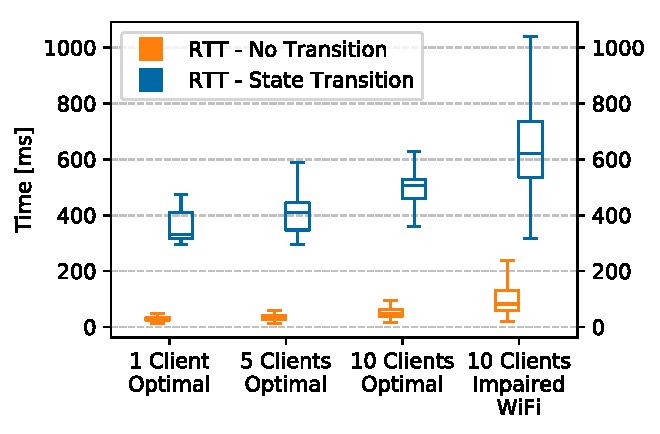
\includegraphics[width=.85\textwidth]{publications/2019EdgeDroid/plots/comparison/nofonts/rtt_fb_vs_nofb}%
    \caption{Comparison of round-trip-times for inputs that triggered a state transition in the task model versus inputs that did not.}%
    \label{fig:comparison:rtt}%
\end{figure}%
\begin{figure}
    \centering%
    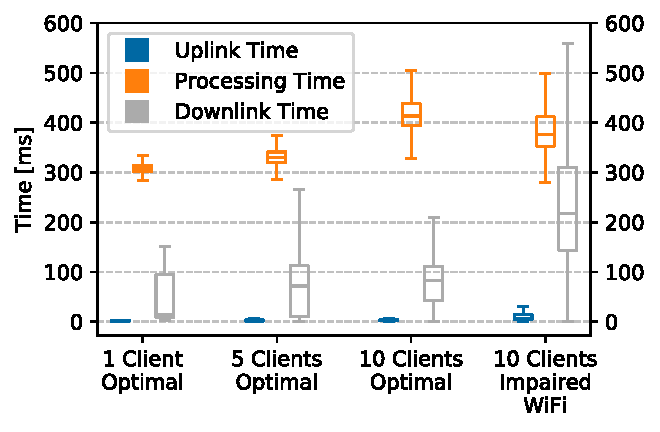
\includegraphics[width=.85\textwidth]{publications/2019EdgeDroid/plots/comparison/nofonts/box_feedback}%
    \caption{Distribution of latency across system components for inputs that triggered a state transition in the task model.}%
    \label{fig:comparison:feedback}%
\end{figure}%
\begin{figure}%
    \centering%
    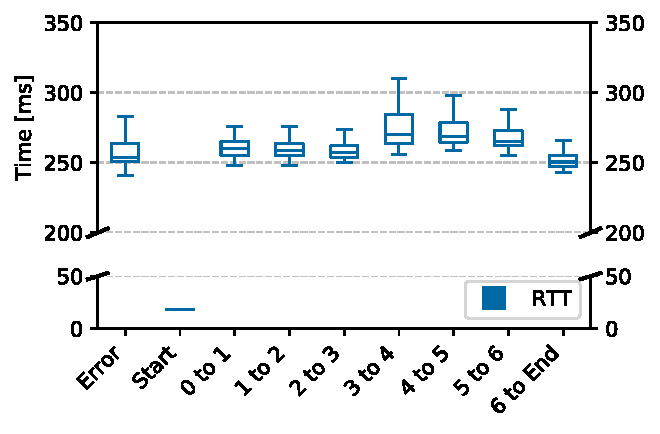
\includegraphics[width=.85\textwidth]{publications/2019EdgeDroid/plots/comparison/nofonts/box_taskstep}%
    \caption{Round-trip-times for input-feedback cycles associated with state transitions in the internal task model for a single client connected over an optimal wireless link.}%
    \label{fig:comparison:tasksteps}
\end{figure}%

The goal of this paper is to provide a methodological approach to studying these latency trade-offs, along with a tool, EdgeDroid 1.0\footnote{We plan to make the EdgeDroid 1.0 benchmarking suite available as Free and Open Source Software and the recorded traces under a Creative Commons License.}, that simplifies the benchmarking of human-in-the-loop applications.
We view EdgeDroid 1.0 to be the very first, and simplest, of a family of tools that will embody increasingly sophisticated and accurate models of user behavior.

Due to the complex nature of the applications and the infrastructure, we opt for experimentally studying the trade-offs in a repeatable and controllable fashion.
This is difficult mainly due to the unpredictable reaction of human users to the feedback from the backend --- a user might very well misinterpret the feedback handed to them.
EdgeDroid 1.0 mimics the operation of human-in-the-loop applications by replaying recorded traces of sensory input.
This sensory information is then processed by the original compute process at the backend, generating feedback.
However, this feedback is not processed by humans, but by a parameterizable model of human reaction.
Through synchronized time tracking at the different processing points of the application, EdgeDroid 1.0 allows for accurate measurements of key performance metrics such as the distribution of delays across the application pipeline.
Analysis of these metrics can be performed down to the individual input sample, allowing us to zoom into the internal model of the application under consideration.
Thus, EdgeDroid 1.0 allows us to illuminate the many latency trade-offs existing at the level of the infrastructure, as well as the level of the application.
It can also be used for debugging and validation, by comparing the expected execution flow of a particular trace with the actual flow during the benchmarking.
To the best of our knowledge, this experimentally-driven benchmarking approach is the first one towards experimental performance characterization and potential optimization of human-in-the-loop applications

\Cref{fig:comparison:rtt} presents a comparison of the total measured round-trip-times (RTTs) both for inputs which caused a state transition and inputs that did not.
Next, \cref{fig:comparison:feedback} shows a comparison of the distribution of latencies across system components for inputs that caused an internal state change in the task model of the application.
We differentiate according to the three main components contributing to latency, namely \emph{uplink} and \emph{downlink transmissions}, and \emph{backend processing}.
Finally, \cref{fig:comparison:tasksteps} depicts the distribution of RTTs for each transition in the internal task model for a single client connected over an optimal wireless link.
These metrics were calculated by recording the measured input-feedback cycle delay corresponding to a change in state within the application.
Thus, for instance, the measurements located at column ``3 to 4'' in the figure correspond to the aggregated round-trip-times for every input-feedback cycle corresponding to a change from state 3 to state 4 within the application task model, for the 100 repetitions of the scenario.

In the following discussion we will refer to inputs which triggered a transition in the task model as \emph{feedback-rich inputs} and those that did not as \emph{feedback-less inputs}.

For the analysis of these results, we will take into consideration the bound of \SI{600}{\milli\second} response time for step-by-step task-guidance derived by the authors of~\cite{Chen:AnEmpiricalStudyOfLatency}.
This bound marks the point after which further delays in the delivery of feedback to the user start to negatively affect user experience, and allows for a straightforward evaluation of the responsiveness of the system.

We will begin our analysis of the experiment results with \Cref{fig:comparison:rtt}.
These results present a stark contrast in the round-trip-times for inputs which cause a state transition versus inputs that do not, with RTTs for the former being up to an order of magnitude greater.
It's worth mentioning though that responses to feedback-less inputs are invisible to the user, and are just included here as a sort of baseline to compare feedback-rich round-trip times with.

We can identify a pair of interesting effects in the scaling of the task-guidance WCA application.
One, scaling behavior for the application seems to be linear with respect to the number of clients.
Two, in the case of the impaired WiFi, the effect on the feedback-rich inputs is very pronounced, with the average of the RTTs for these inputs being over the previously discussed bound of \SI{600}{\milli\second}.

It is worth noting that already at just 10 clients the response times for feedback-rich inputs are very close to the bound.
Looking at this through the lens of a an application developer, it could hint at a need for optimization of the later parts of the application pipeline, since RTTs for inputs which are discarded in the detection stage of the pipeline (i.e.\ feedback-less inputs) are still well below \SI{200}{\milli\second}.

EdgeDroid 1.0 allows researchers to zoom into specific components of the application feedback loop, as exemplified by \cref{fig:comparison:feedback}.
From this figure it is clear that the main component which contributes to latency in the optimal case is the backend processing, further lending credibility to our previous comment on the need for optimization.
Nevertheless, when the link quality decreases, the delays on the downlink start to overshadow the delays on the processing.
Here, the downlink time sometimes almost reaches the ideal bound by itself.
A system designer might then conclude from this that in order to be able to scale the application, their focus needs to be on improving the quality of the wireless link before increasing the processing power on the backend.

Finally, EdgeDroid 1.0 allows even more insights to be gained by homing in to individual steps in a task-guidance WCA. Consider \cref{fig:comparison:tasksteps}.
The figure shows clears spikes in latencies at the transitions from task state 3 to 4 and from task state 4 to 5, which could indicate to the application developer that these specific transitions are ripe for optimization.


\todo[inline]{\cref{paper:olguinmunoz2019edgedroid}}\label{summary:2019edgedroid}

\subsection{Applying the methodology to \acsp{NCS}}\label{ssec:methodology:ncs}

\todo[inline]{\Cref{paper:olguinmunoz2022cleave} implements both the methodology and the tool.}

\begin{figure*}
    \centering
    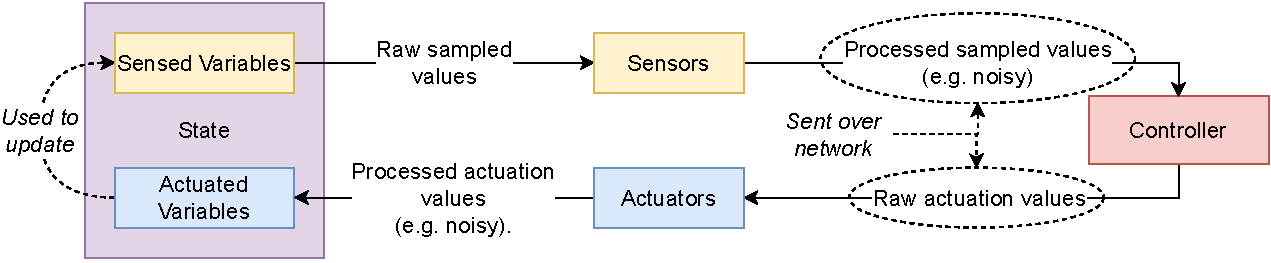
\includegraphics[width=.8\textwidth]{publications/2022CLEAVE/images/CLEAVE_NCS_structure}
    \caption{
        Structure of an emulated \acl*{NCS} in \acs*{CLEAVE}.
    }\label{fig:cleave:ncs:struct}
\end{figure*}

We overcome this issue by proposing a completely virtual plant allowing for unparalleled flexibility in changing the plant model and characteristic features of the experiments.
In this paper, we present the first fully-software-based framework for scalable and repeatable benchmarking of edge-native \ac{NCS}.
As edge computing begins being adopted by industry, more and more variations have begun to appear in literature.
``Near'', ``far'', ``core'', and ``telco'' edge describe variations of the original concept and are becoming ubiquitous in new research.
While the core idea of edge computing is widely accepted as fundamental for pervasive \acp{NCS} in general, understanding the strengths and weaknesses of such different edge concepts is of paramount importance.

Our framework, \ac{CLEAVE}, aims to simplify the repeatable and scalable benchmarking of such systems.
It is fully virtualized, inspired by our previous work on benchmarking human-in-the-loop applications on the edge~\cite{Olguin2019EdgeDroid}.
The tool consists of a benchmarking framework and software development kit for the development of emulated physical systems and softwarized controllers.
These virtual \acp{NCS} can then be deployed on real networks for reparametrizable, repeatable, and reproducible benchmarking of the complete system.

\ac{CLEAVE} is built using \emph{Python 3.8}, making it highly extensible and able to harness the multitude of already existing user libraries.
It is furthermore compatible with container technologies such as \emph{Docker}\footnote{Docker Engine: \url{https://www.docker.com/}}, making it suitable for automated deployment, scaling, and benchmarking on industry-standard edge setups using container orchestration solutions.

In this work, we aimed to tackle this issue through a fully software-based framework for repeatable, reproducible, and easily scalable \ac{NCS} benchmarking with a particular focus on edge deployment.
We argue our approach, \ac{CLEAVE}, embodies a better solution than previous work for a number of reasons:
\begin{enumerate}
    \item Compared to fully physical approaches, such as those used in\ \cite{Baumann2018LowPower} and\ \cite{Cuenca2019UAV}, our approach allows for greater flexibility and scalability.
          The aforementioned approaches rely on specialized and sometimes entirely custom-built physical platforms, and although flexible and cheap approaches such as Zoppi \emph{et al.'s} --- which uses a LEGO-based physical plant --- exist, these still do not reach the level of flexibility afforded by a fully software-based framework.
          Experimenters still need copies of the hardware, making anything other than small-scale setups unfeasible.
          In contrast, our approach requires only general-purpose computing platforms, and can be employed by basically anyone with access to a computer.
          Scalable deployments can in turn easily and cheaply be set up using single-board computers and/or virtual cloud instances.
    \item When compared to simulated approaches such as\ \cite{Ma2019DynamicSched}, \ac{CLEAVE} provides a higher level of realism, in particular with regards to the network segment of the system.
    \item Finally, although it shares much in common with previous emulated approaches such as the one employed in\ \cite{Wang2020VoltageControl}, \ac{CLEAVE} has an advantage by specifically targeting a general-purpose approach using industry-standard, cloud- and edge-native tools and software.
          The tool can easily be deployed and scaled using widely-used frameworks such as Docker Swarm and Kubernetes.
\end{enumerate}

We validate the utility of this tool through an example use case approximating a proposed edge deployment of inverted pendula control loops co-located with video analytics services.
We argue such a use case represents a realistic scenario and appropriate benchmark for the tool, since
\begin{enumerate*}[itemjoin={{; }}, itemjoin*={{; and }}]
    \item the inverted pendulum plant is ubiquitous in \ac{NCS} research
    \item similar setups exist in real-world industrial use
    \item video analytics has long been proposed as a ``killer app'' for edge computing.
\end{enumerate*}
Our results showcase the ability of the framework to extract relevant metrics relating to the stability of the control system, as well as on the performance of the underlying network link.
We believe \ac{CLEAVE} represents an important step towards enabling inexpensive and low-complexity scalable research for real-world deployment of edge-bound \acp{NCS}.

\todo[inline]{Some plots and results}

\begin{figure}
    \centering
    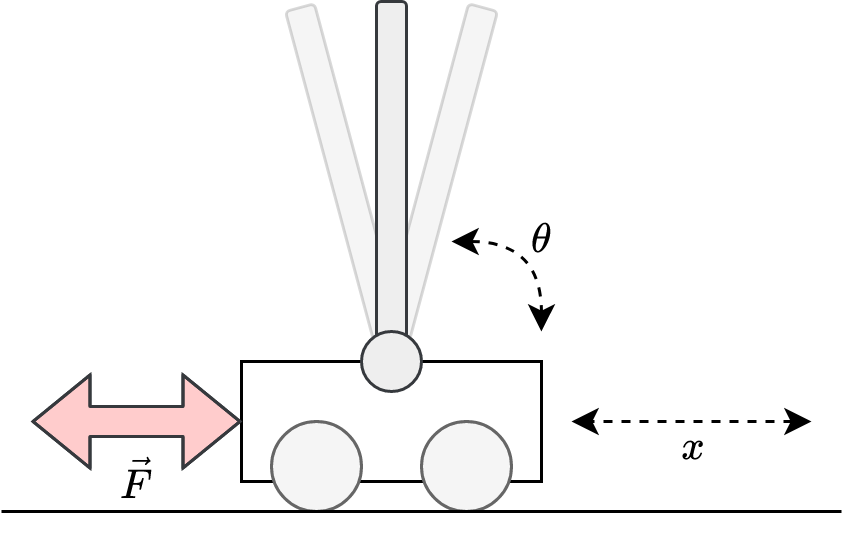
\includegraphics[width=.6\textwidth]{publications/2022CLEAVE/images/inverted_pendulum.png}
    \caption{
        The 2D inverted pendulum system.
    }\label{fig:invpend}
\end{figure}

\begin{figure}[t]
    \centering
    \begin{subfigure}[h]{.22\textwidth}
        \centering
        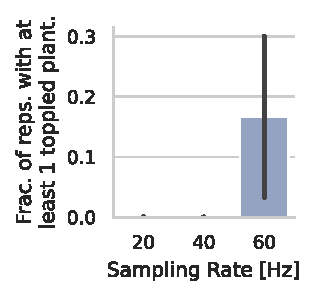
\includegraphics[width=\textwidth]{publications/2022CLEAVE/plots/fixed_video_topple_frac}
        \caption{Toppled plants.}\label{fig:video:toppled}
    \end{subfigure}%
    \hfill%
    \begin{subfigure}[h]{.22\textwidth}
        \centering
        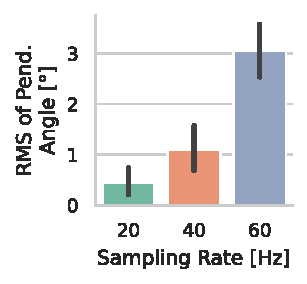
\includegraphics[width=\textwidth]{publications/2022CLEAVE/plots/fixed_video_angle_rms}
        \caption{Angle \ac{RMS}.}\label{fig:video:rms}
    \end{subfigure}\\
    \begin{subfigure}[h]{.22\textwidth}
        \centering
        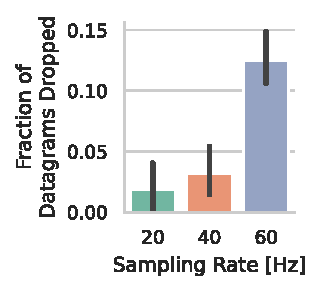
\includegraphics[width=\textwidth]{publications/2022CLEAVE/plots/fixed_video_drop_frac}
        \caption{Packet losses.}\label{fig:video:drop}
    \end{subfigure}%
    \hfill%
    \begin{subfigure}[h]{.22\textwidth}
        \centering
        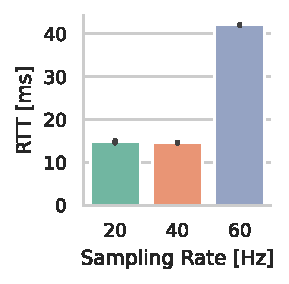
\includegraphics[width=\textwidth]{publications/2022CLEAVE/plots/fixed_video_rtt}
        \caption{\acsp{RTT}.}\label{fig:video:rtt}
    \end{subfigure}%
    \caption{
        Multi-loop, resource-constrained setup results.
        Error bars indicate \SI{95}{\percent} \acp{CI} in all plots.
    }\label{fig:video:results}
\end{figure}

\FloatBarrier%

\subsection{Orchestrating experimentation in edge computing testbeds}

\todo[inline]{\cref{paper:olguinmunoz2022ainur} describes a software framework for testbeds used for the methodology described in this thesis}

In this work, we present our solution to the challenge of testbed automation: Ainur, a framework for wireless testbed automation with a specific focus on end-to-end experimental research in the context of edge-computing using cloud- and edge-native technologies.
Ainur is designed to deploy experimental runs from a workload perspective by configuring the physical testbed, initializing all involved software components, deploying and executing the experimental workload, collecting logs and data, and finally gracefully degrading the system.
The framework allows for dynamic, software-definition of physical and logical links, network topology, cloud and edge computing resources, as well as experimental workload deployment and orchestration.
It heavily leverages cloud-native technologies, such as Docker containers, in order to support a wide variety of different testbed hardware setups and experimental configurations and workloads, as well as to be as easily extendable as possible.
Furthermore, we make Ainur available to the community as \ac{FOSS}.
It can be obtained from the {KTH-EXPECA/Ainur} repository on GitHub~\cite{ainur:github}, released under an Apache version \num{2.0} license.

In this paper, we have introduced a framework for repeatable end-to-end testbed automation in the context of wireless networking and edge computing research.
Named Ainur, it simplifies the execution and verification of end-to-end experimentation by automating the
\begin{enumerate*}[itemjoin={{; }}, itemjoin*={{; and }}]
    \item establishment of physical links between hosts, including the configuration of complex wireless systems such as 4G \ac{LTE} and 5G
    \item provisioning of and connection to remote cloud instances
    \item initialization of \ac{IP} layer connectivity between hosts
    \item collection of logs and data
    \item deployment, scaling, and lifecycle management of containerized processes
\end{enumerate*}.
We have described its general architecture, which follows a layered design mimicking the network stack layers the framework directly interacts with, as well as the underlying assumptions about its deployment environment and specific requirements for its deployment.
We have also outlined a demonstration which showcases the flexibility and power of the framework by deploying two different workloads to our testbed.
We believe our framework represents an important step towards repeatable, replicable, yet low-access barrier end-to-end wireless testbed experimentation.
It has been released as \ac{FOSS} and can be found on GitHub~\cite{ainur:github}.\\

\todo[inline]{Some plots}

\begin{figure}[t]
    \centering
    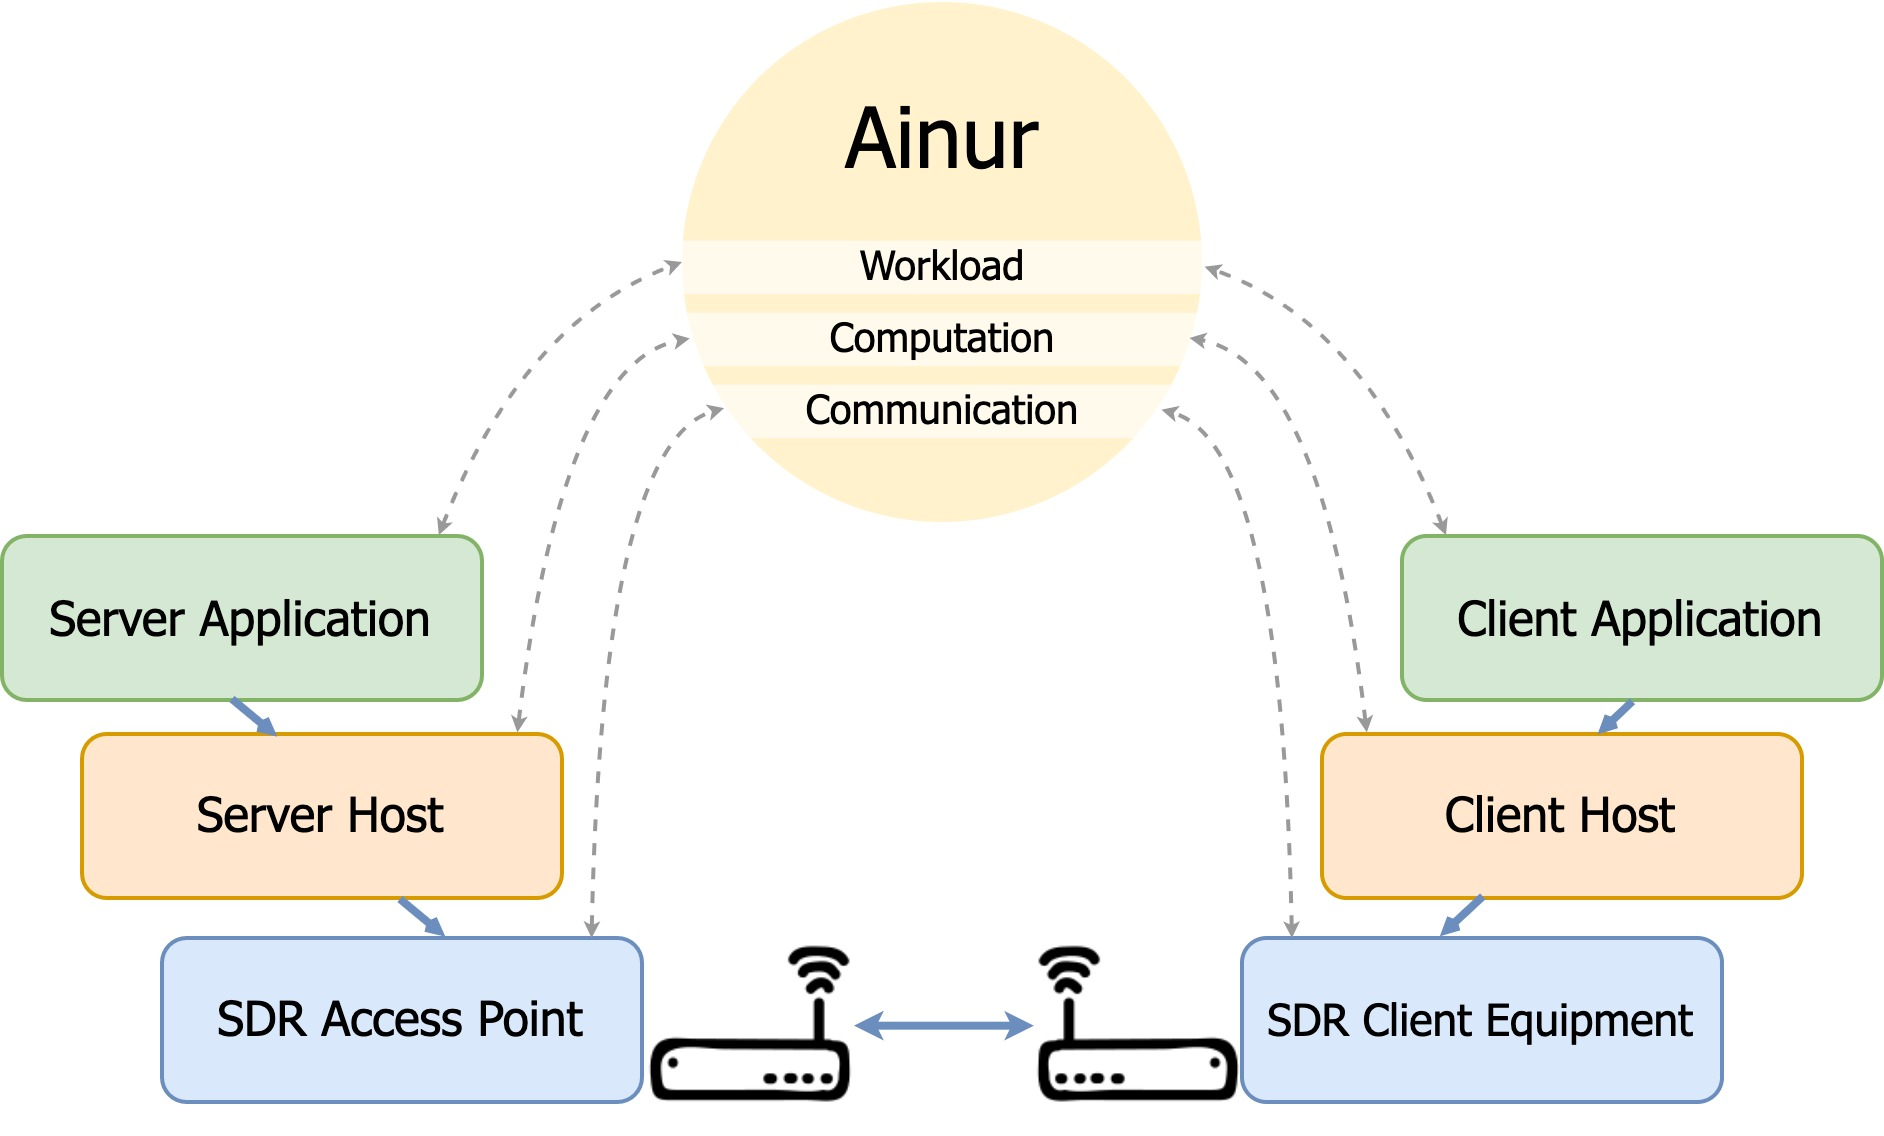
\includegraphics[width=0.9\linewidth]{publications/2022Ainur/figures/overview.jpg}
    \caption{Layered structure of an Ainur experiment}\label{fig:overview}
\end{figure}

\begin{figure*}
    \centering
    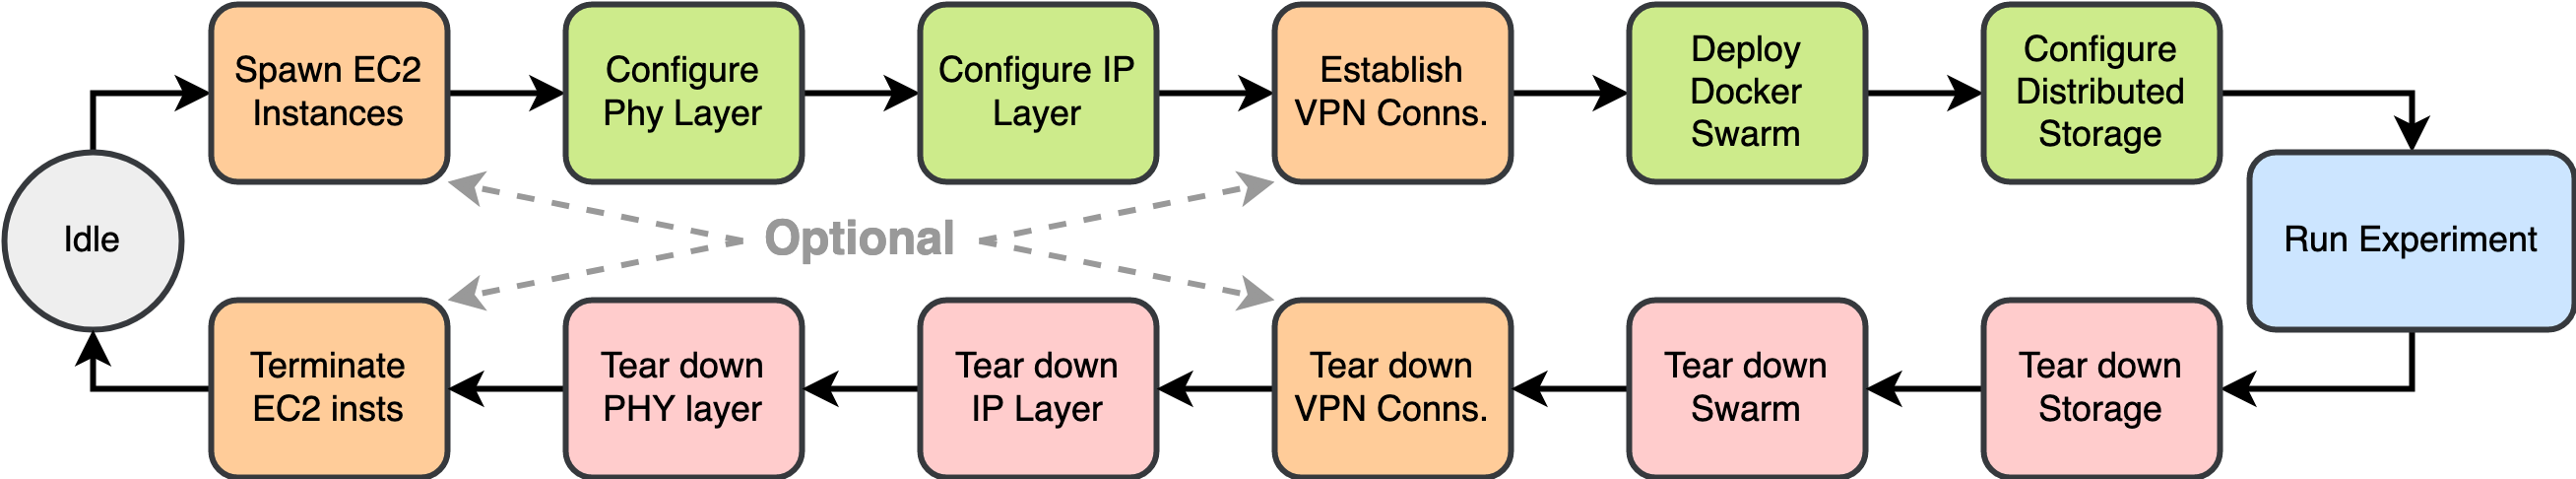
\includegraphics[width=0.8\textwidth]{publications/2022Ainur/figures/flow2.png}
    \caption{Lifecycle of an experimental run in Ainur. Blocks in orange are optional.}\label{fig:flow}
\end{figure*}

\begin{figure*}
    \centering
    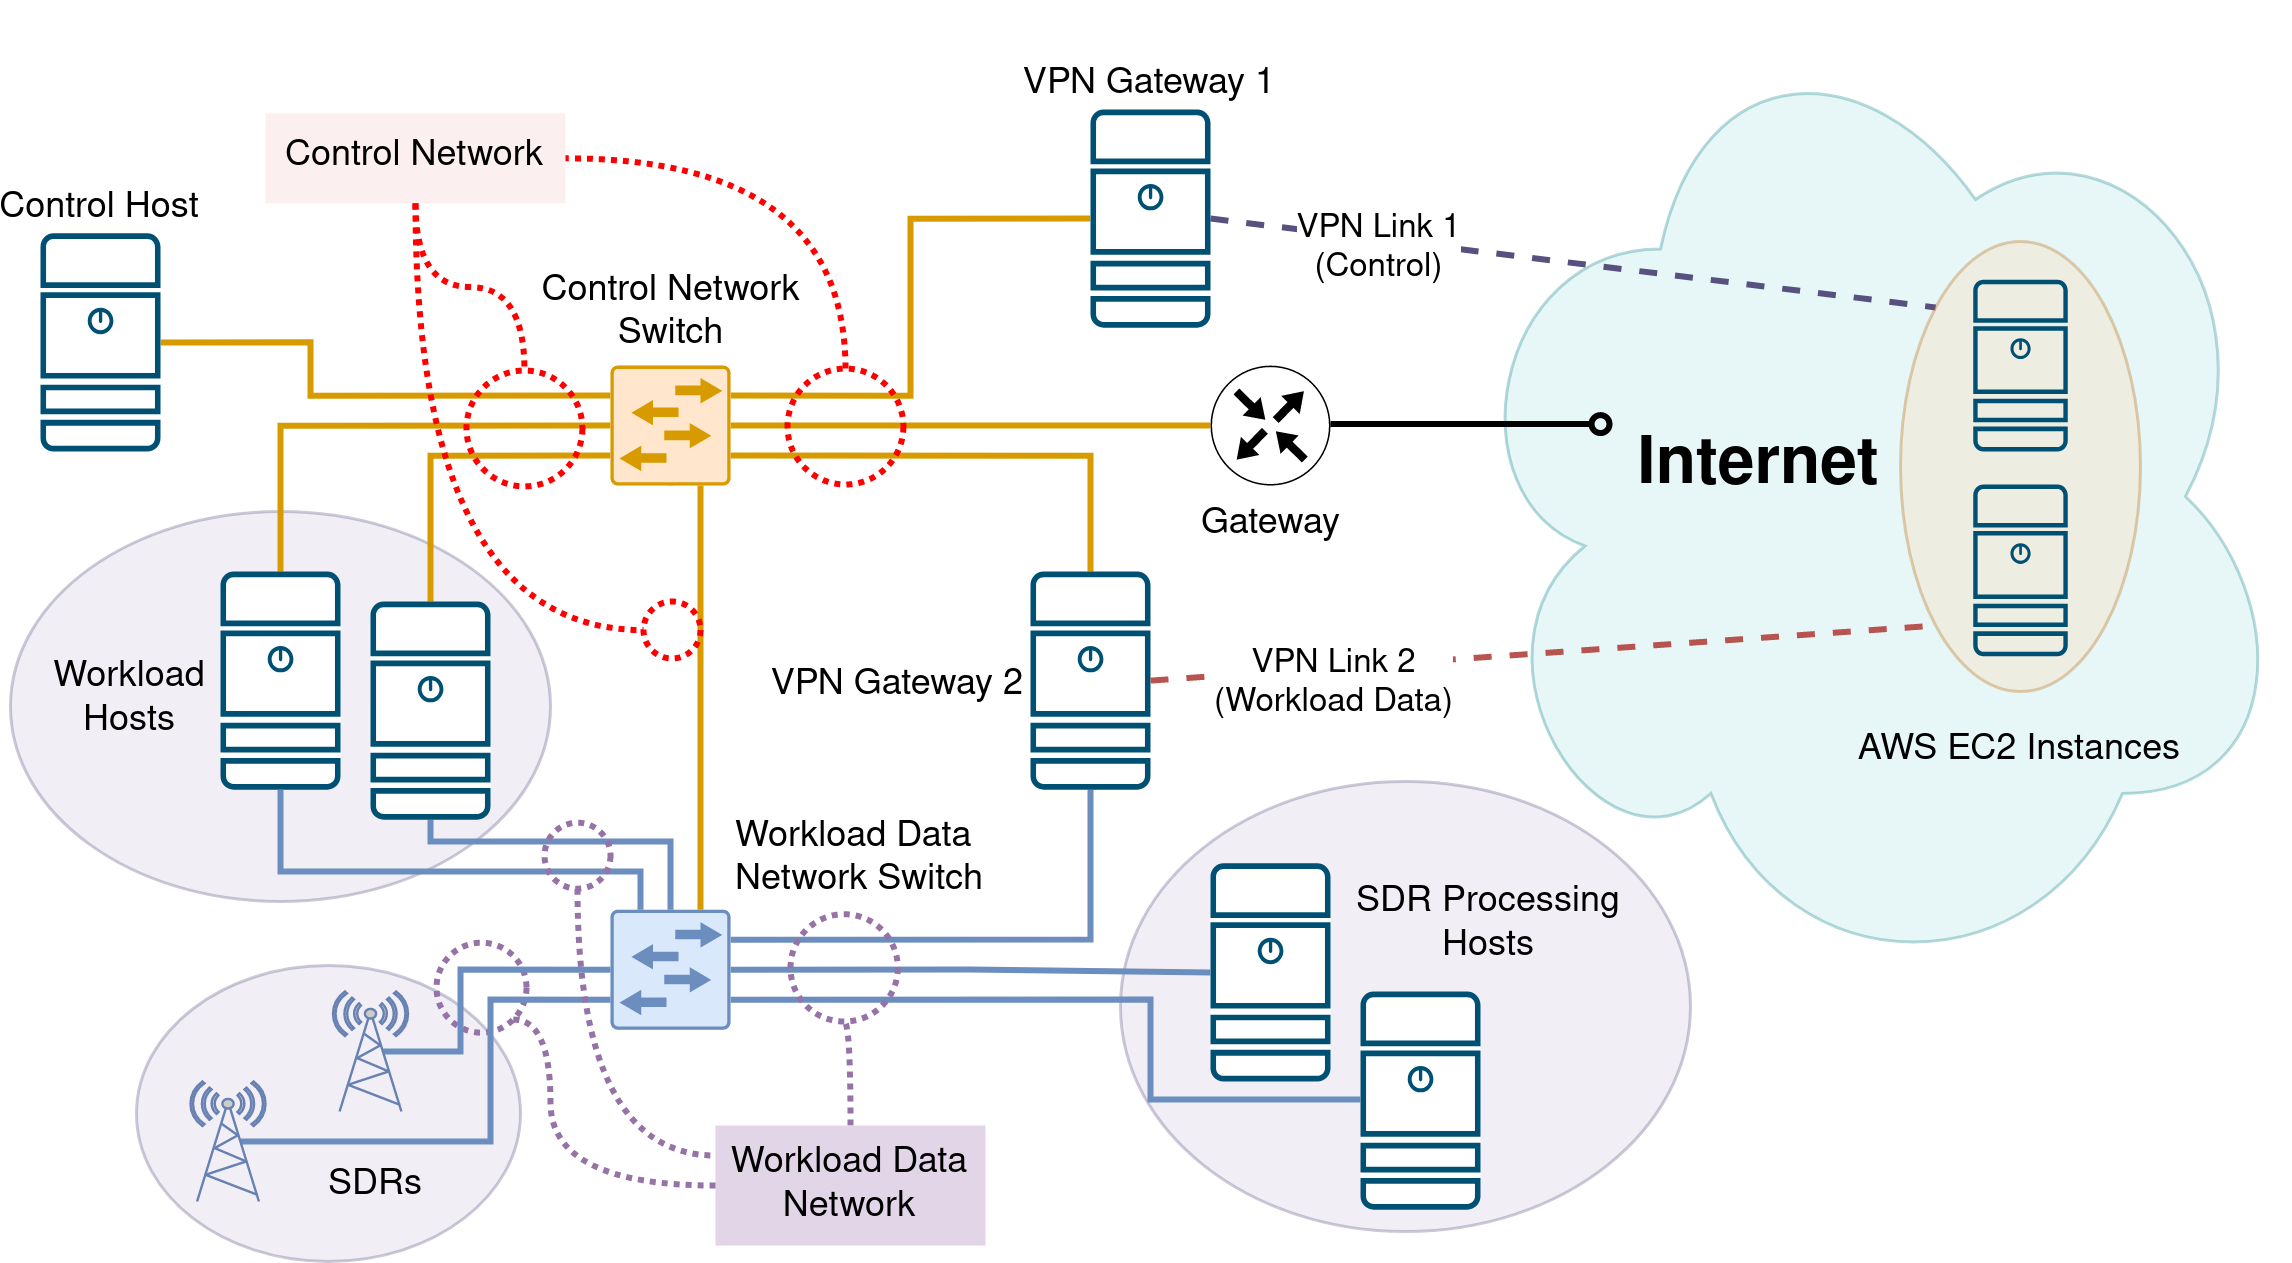
\includegraphics[width=.8\textwidth]{publications/2022Ainur/figures/network.png}
    \caption{Network structure assumed by Ainur.}\label{fig:network}
\end{figure*}

\section{Extending the methodology in the context of \acs{WCA}}

\subsection{Characterizing human behavior}

\todo[inline]{\cref{paper:olguinmunoz2021impact} describes the acquisition of the necessary data and insights for the models.}

\todo[inline]{From introduction}

We intended to answer four core research questions relating to human responses to decreased application responsiveness.

\begin{itemize}
    \item \emph{Do subjects change the temporal profile of their actions in relation to system latency?}

          In line with previous research in this area, we expected subjects to change their temporal profiles as system responsiveness decreased.
          The extent or form of these changes were however unknown.
          We also hypothesized that large enough drops in responsiveness could lead to complete abandonment of the task by subjects.

          Our results show an emergent pacing effect on user actions as system responsiveness is reduced.
          While it would seem self-evident that users take longer to complete a task while using a system with low responsiveness --- as they have to wait longer for new instructions --- our study found that user slow-down represents a source of substantial additional delay.
          To be more precise, the data indicate that users slow down not only because they have to wait for the system to catch up, but that their reactions to new instructions is also delayed.
          Moreover, this effect scales with the decrease in responsiveness and remains for a while, even after system responsiveness improves.

    \item \emph{Do subjects show signals of arousal in physiological responses to changes in system latency?}

          We hypothesized subjects would show signs of stress and frustration as system latency increased, due to the added annoyance of dealing with an unresponsive system.

          The results we present, however, seem to refute this hypothesis.
          We were not able to detect any significant effects on the physiological signals obtained from the biometric sensors as system responsiveness was altered.

    \item \emph{Are responses to delay effects in subjects mediated by cognition and/or emotion?}

          In line with previous items, we expected delay effects in subjects to be mediated primarily by emotion.
          In particular, we expected emotional effects to be correlated with the strength of the added delay.

          The results point in a different direction though, indicating that reduced responsiveness in WCA systems leads to a disruption of participants' cognitive plan for the task and not to an emotional response.
          This is evidenced by the previously discussed pacing effect and the lack of significant physiological responses.

    \item \emph{Are these effects mediated by personality indicators in any way?}

          Finally, we hypothesized that the individual trait of \emph{neuroticism}~\cite{john1999:bfi} would play a role in mediating these effects, as it has previously been connected to intolerance for time delay~\cite{hirsh2008delay}.
          We also expected \emph{focus} and \emph{involvement}~\cite{witmer1998:itq} to play roles in this.

          The results obtained agree with our hypothesis.
          We found significant effects of neuroticism on the responses exhibited by subjects, and all three traits were found to play a role through factor analysis.

\end{itemize}

% Our results indicate that reduced responsiveness in WCA systems leads to a disruption of participants' cognitive plan for the task.
% This is evidenced by an emergent pacing effect on user actions as system responsiveness is reduced.
% While it would seem self-evident that users take longer to complete a task while using a system with low responsiveness --- as they have to wait longer for new instructions --- our study found that user slow-down represents a source of substantial additional delay.
% To be more precise, the data indicate that users slow down not only because they have to wait for the system to catch up, but that their reactions to new instructions is also delayed.
% Furthermore, this effect persists for a while after system response improves and is modulated by intrinsic personality traits, in particular, \emph{neuroticism}~\cite{john1999:bfi}. 

We believe that these results provide concrete and relevant implications for WCA design, deployment, and optimization.
One example is the behavioral slow-down, as it extends application runtime significantly, and thus has clear and direct implications for resource and power consumption.
Another is the fact that the adverse effects of delay on users do not immediately subside as delay is diminished --- this has potential consequences for resource allocation strategies.
Moreover, in multi-user scenarios, the dependency of user slow-down effects on delay mean efficient resource allocation across applications potentially looks different from what could be considered ``fair''.

Our hope is that the results we provide might prove useful for the understanding and optimization of deployments of WCA.\@
These results represent unexpected, valuable findings, which can be employed to model and understand how users interact with latency in applications and systems, and develop resource allocation and power optimization strategies.
Additionally, we hope that the results we provide might pave the way for the improvement of performance evaluation tools such as our previous work in \cite{olguin:2018, olguin:2019}.
Such systems would greatly benefit from this knowledge, as it would allow for the design and implementation of realistic models of human behavior, making highly accurate benchmarks a reality in the domain of WCA.\@

\todo[inline]{From discussion}

We start our discussion with the main results of our experimentation presented in the previous section:

\begin{itemize}
    \item Firstly, and perhaps most importantly, we find that a system slow-down induces an \textit{additional} behavioral slow-down.
          That is, as system responsiveness decreases, our data indicates that users significantly slow-down in their execution of the task.
          This slow-down scales with the decrease in responsiveness; compared to the no-delay case, participants were on average \SI{12}{\percent} slower at \SI{1.65}{\second} delay and \SI{26}{\percent} at \SI{3.0}{\second} delay.
          Moreover, there is a temporal component to this effect; users become progressively slower the more time passes with reduced system responsiveness.

    \item Secondly, we find that the effects of behavioral slow-down due to impaired system responsiveness \emph{remain} for at least a few steps after system responsiveness improves.
          This is evidenced by the longer per-step-execution times of the first four steps of blocks immediately following a high-delay block, as pictured in \cref{fig:exectime:transition}.
          The question of whether any lingering effect can be measured after these four steps remains open.

    \item Thirdly, we evidence a speed-up in execution time over a series of steps; that is, subjects get faster at performing steps as the task progresses.
          However, the strength of this effect decreases as delay increases.
          Whereas for blocks without delay users performed the last four steps of a 12-step block on average \SI{36}{\percent} faster than the first four, at the maximum delay this effect practically disappears.

    \item Fourthly, in terms of inter-subject differences, PCA revealed three main factors governing users' response to delay.
          The first factor represents sensitivity to delay as moderated by the ``Big Five'' personality trait of neuroticism and both measures of immersion: focus and involvement.
          Factor two and three represent dedication to the task as opposed to delay intolerance and reflect variables related to attentiveness, respectively.
          In simple terms, these results suggest that the effects of delay are most potent in individuals who are sensitive and involved in the task.
          The findings appear selective to cognitive assistance tasks like the present ones, inasmuch as the same measures did not correlate with outcomes in other computer-intensive environments such as immersive VR~\cite{quesnel2018you}.
          These correlations are also consistent with previous findings indicating that individuals scoring high in neuroticism tend to be intolerant to delayed reward~\cite{hirsh2008delay}.
\end{itemize}

A central question therefore arises: to which physio- and psychological mechanisms can these findings, most importantly the substantial slow-down in task execution, be attributed?

In \cref{sec:background}, we initially considered the possibility that delays might produce negative emotional reactions.
These could in turn elicit generalized arousal.
We also postulated that adapting to delay might progressively deplete cognitive resources in users.
However, the present data provide relatively little support for these alternatives, in that the predicted measures did not produce the expected statistical trends.
Specifically, physiological measures of GSR and HR failed to show evidence of differential arousal under long vs.\ short delays, and speed-induced errors and non-completions predicted by resource depletion were not observed.
The acceleration data further did not indicate that extended delay significantly increases erratic movement.
% physiological measures of GSR and HR failed to show evidence of differential arousal under long vs.\ short delays, and speed-induced errors and non-completions predicted by resource depletion were not observed.
% The acceleration data further do not indicate that extended delay increases erratic movement.
To the contrary, the data suggest this effect results from a delay in movement after an instruction is introduced.
That is, users fail to capitalize on the new information as quickly as they could.
Thus, contrary to our preliminary postulations, behavioral effects seem to arise from impaired cognitive control mechanisms, and not from emotion or resource depletion.
We hypothesize that the effects of feedback latency can best be understood as changes in the use of a cognitive plan.
As was described in \cref{sec:experimentaldesign,fig:lego:hierarchical}, complex cognitive and motor tasks have been modeled as the unfolding of a hierarchy of command, from high-level plans to physical output.
Long system latencies, we propose, disrupt the automating of such a plan, instead relegating it to attention-based control at the step-by-step level that is easily diverted.
This also provides a possible explanation for the lingering effects of delay after an acceptable system responsiveness is restored, as users needs time re-adjust and re-automate their cognitive plans.

As to the applicability of our findings to other applications, it must be noted that these results pertain to a specific class of applications, namely step-based task-guidance WCA.\@
However, we would expect our findings to extend to similar applications, as long as they follow the same pattern of seamless interaction --- i.e.\ such that the user does not need explicitly interact with the application to advance the state.

The results here presented provide a number of possible implications for WCA system design and optimization, both for single and multi-application flows.

\begin{itemize}

    \item Due to the behavioral slow-down in users, even short-term reductions in responsiveness will lead to significantly extended application lifetimes.
          This has direct implications for resource and power consumption.

    \item The fact that the adverse effects of delay on users do not immediately disappear as the system returns to a high-responsive state could have unconventional consequences for resource allocation.
          This is of particular importance, for instance, for cases where the user may be able to finish the task before these effects subside.
          In such cases, the limited potential gains might not justify diverting valuable system resources to the impaired application.

    \item In multi-user environments, the time dependency of user slow-down effects mean that fair degradation of system responsiveness across applications may not ultimately be beneficial to the system as a whole.
          Take for instance two applications on the same system which negatively interfere with each other.
          The longer they interfere with each other, the longer their respective lifetimes are going to be, which in turn causes them to interfere even longer, potentially entering a positive feedback loop.
          In such a case, prioritizing one over the other rather than trying to improve responsiveness for both might lead to resources being freed up faster system-wide.

    \item Based on our findings relating individual differences between users and their sensitivity to delays, it might also be possible to extrapolate user characteristics from measured execution times.
          This could prove a valuable tool for load balancing, for instance by prioritizing resource allocation to users with a higher sensitivity to system-state degradation.
          However, this remains an open challenge.

\end{itemize}

To wrap up, we believe the present data provide novel and unexpected insights for the understanding and optimizing of WCA deployments.
Although more subtle than expected, and in some cases somewhat counterintuitive, these insights represent a valuable tool to tackle inefficiencies in these systems.
Moreover, we also argue these findings represent a first step towards a full-fledged understanding of the relationship between application responsiveness and human behavior.
More research in this area will surely uncover more complex and interesting behaviors.
Finally, we believe the data provide parameters that can usefully be integrated into cognitive models of WCA that might be constructed under existing architectures like ACT-R.
These same parameters could be used to modulate the timing and generation of inputs in trace-based workload generation tools such as the EdgeDroid platform~\cite{olguin:2018,olguin:2019}, allowing the tool to use the same trace to generate workloads for a multitude of different user profiles.

\todo[inline]{Some diagrams, plots, and results}

\begin{figure}[h]
    \centering
    \begin{subfigure}[t]{.49\textwidth}
        \centering
        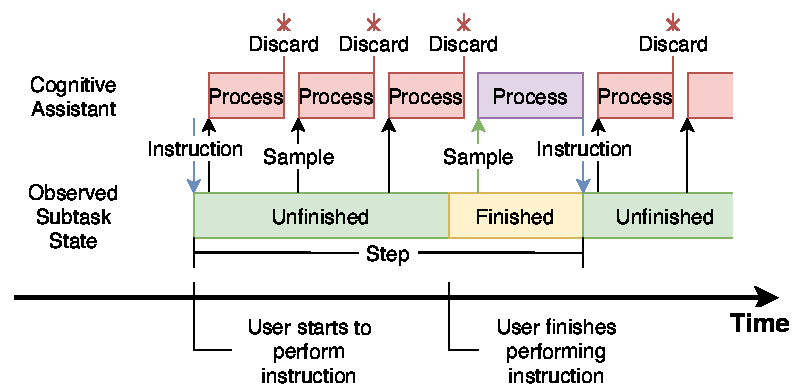
\includegraphics[width=\textwidth]{publications/2021ImpactDelayedResponse/Fig4a.eps}
        \caption{Structure of a step in a generic cognitive assistance application.
            The assistant provides an instruction to the user and continuously samples the step state; inputs captured while the step is unfinished are silently ``discarded'' (i.e.\ they do not cause the generation of a new instruction).
            % by the assistant, as they do not contain relevant information.
            Once the user finishes performing the step, the next sample \emph{will} cause the generation of a new instruction.
            % which will subsequently be provided to the user.}%
        }
        \label{fig:cogassist:step}
    \end{subfigure}%
    % \medskip%
    \hfill%
    \begin{subfigure}[t]{.49\textwidth}
        \centering
        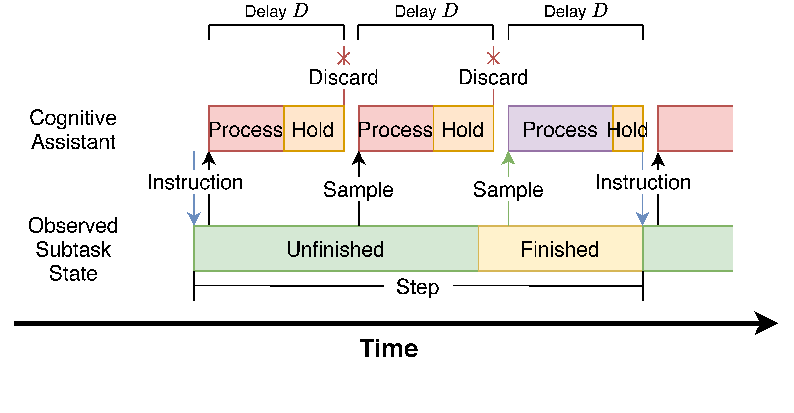
\includegraphics[width=\textwidth]{publications/2021ImpactDelayedResponse/Fig4b.eps}
        \caption{In the experimental task, an additional variable segment of time is introduced immediately following the processing of the input frame in order to extend the perceived processing time of the input to a specific target delay.}%
        \label{fig:cogassist:step:delay}
    \end{subfigure}
    \medskip%
    \begin{subfigure}[t]{.49\textwidth}
        \centering
        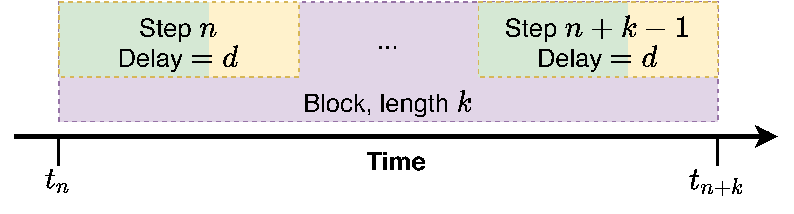
\includegraphics[width=\textwidth]{publications/2021ImpactDelayedResponse/Fig4c.eps}
        \caption{Structure of a block in the experimental task.}%
        \label{fig:cogassist:block}
    \end{subfigure}%
    % \medskip%
    \hfill%
    \begin{subfigure}[t]{.49\textwidth}
        \centering
        \includegraphics[width=\textwidth]{publications/2021ImpactDelayedResponse/Fig4d.eps}
        \caption{Visualization of the execution time of a step.}%
        \label{fig:exectime:diagram}
    \end{subfigure}%
    % \medskip%
    \caption{Components of the cognitive assistance task.}
\end{figure}

\begin{figure}[h]
    \centering
    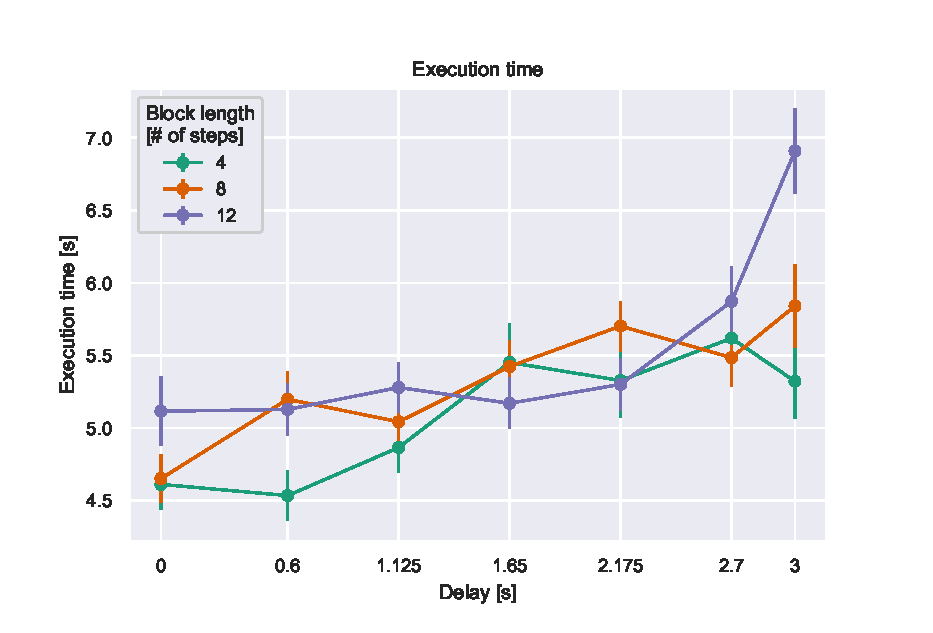
\includegraphics[width=.8\textwidth]{publications/2021ImpactDelayedResponse/Fig6.eps}
    \caption{Per-step execution time by block length vs.\ delay. Error bars indicate the Standard Error of the Mean (S.E.M.)}\label{fig:exectime}%    
\end{figure}

\begin{figure}[h]
    \centering
    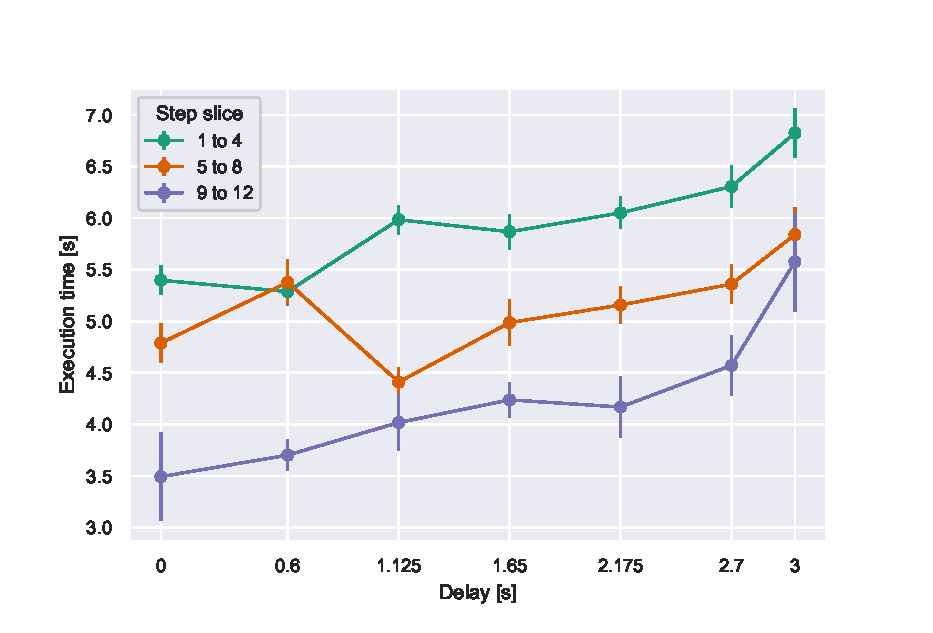
\includegraphics[width=.8\textwidth]{publications/2021ImpactDelayedResponse/Fig7.eps}
    \caption{Mean per-step execution time vs.\ delay, by step slice.
        Error bars indicate S.E.M.}
    \label{fig:exectime:delay:slice}
\end{figure}

\begin{figure}[h]
    \centering
    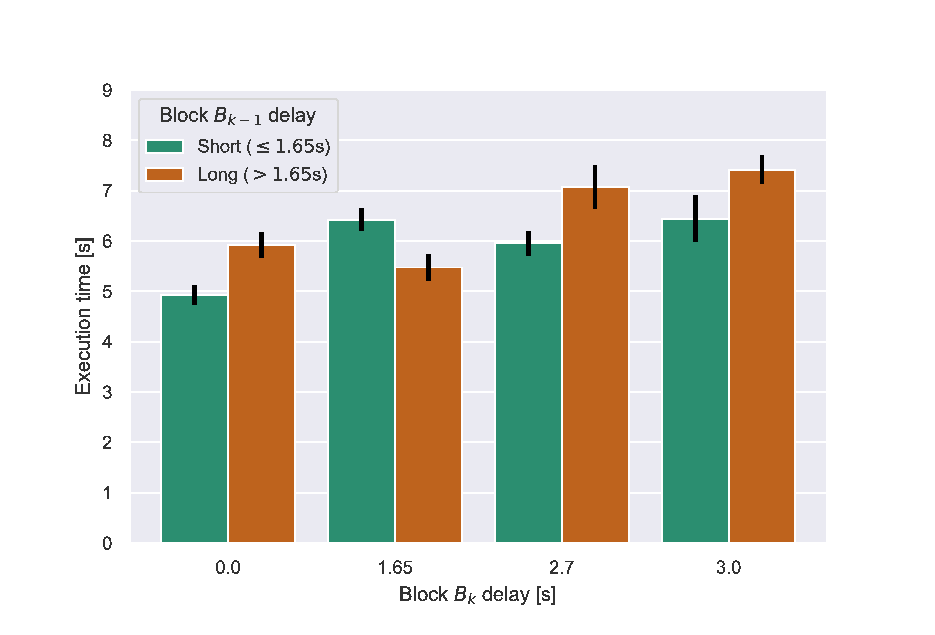
\includegraphics[width=.8\textwidth]{publications/2021ImpactDelayedResponse/Fig8.eps}
    \caption{Per-step execution time across the first four steps after a block transition from block \( B_{k-1} \) to \( B_k \). Error bars indicate S.E.M.}\label{fig:exectime:transition}%
\end{figure}

\begin{table}[h]
    \centering
    \caption{Principal Component Analysis}\label{tab:pca}
    \begin{subtable}[h]{\textwidth}
        \centering
        \caption{Main components identified.}
        \setlength{\tabcolsep}{0pt} % let TeX compute the intercolumn space
        \begin{tabular*}{\textwidth}{@{\extracolsep{\fill}\quad}lrrr@{}}
            \toprule
            \textbf{Factor} & \textbf{Comp. 1} & \textbf{Comp. 2} & \textbf{Comp. 3} \\
            \midrule
            BFI Conscientiousness                  & \textcolor{lightgray}{\( -0.022 \)} &                         \( 0.668 \) & \textcolor{lightgray}{\( -0.481 \)} \\
            BFI Neuroticism                        &                         \( 0.600 \) &                        \( -0.678 \) & \textcolor{lightgray}{\( -0.118 \)} \\
            ITQ Focus                              &                         \( 0.678 \) &  \textcolor{lightgray}{\( 0.203 \)} &                         \( 0.504 \) \\
            ITQ Involvement                        &                         \( 0.573 \) &                         \( 0.540 \) &  \textcolor{lightgray}{\( 0.417 \)} \\
            Exec. Time (delay 3.0 s, length 12)    &                         \( 0.758 \) & \textcolor{lightgray}{\( -0.178 \)} & \textcolor{lightgray}{\( -0.348 \)} \\
            Log EEG power \( \alpha + \beta \) Slice 1 & \textcolor{lightgray}{\( -0.436 \)} & \textcolor{lightgray}{\( -0.251 \)} &                         \( 0.589 \) \\
            \bottomrule
        \end{tabular*}
    \end{subtable}
    \newline
    \medskip
    \newline
    \begin{subtable}[h]{\textwidth}
        \centering
        \caption{Percentages of variance explained by the components.}
        \begin{tabular*}{\textwidth}{@{\extracolsep{\fill}\quad}lrrrr@{}}
            \toprule
            {} & \textbf{Comp. 1} & \textbf{Comp. 2} & \textbf{Comp. 3} & \textbf{Total} \\
            \midrule
            Explained Variance & \SI{31.88}{\percent} & \SI{22.22}{\percent} & \SI{19.03}{\percent} & \SI{73.13}{\percent} \\
            \bottomrule
        \end{tabular*}
    \end{subtable}
\end{table}

\subsection{Emulating human behavior}

We introduce the first, to our knowledge, data-driven model for human timings in \ac{WCA} applications.
Using the data collected for \textcite{olguinmunoz:impact2021} as a base, we build a stochastic model which takes as input past measurements of system responsiveness and produces realistic step execution times.
We also introduce a novel way to generate dynamic traces of frames for \ac{WCA} applications which can be combined with the timing model for a full end-to-end emulation of a human.
We name this new model \emph{EdgeDroid 2.0}; a direct, more realistic evolution of our initial EdgeDroid approach~\cite{olguin2018scaling,olguin2019edgedroid}.

The study and benchmarking of \ac{WCA} applications is a challenging discipline due to these application's intrinsic human-in-the-loop nature.
Humans are notoriously unreliable, and greatly complicate the scalability and repeatability of experiments.
Furthermore, recruiting large enough cohorts of humans for large-scale experimentation is both greatly time-consuming and prohibitively expensive for many research groups.

In the first half of this paper, we have introduced the EdgeDroid 2.0 model of human timing behavior for \ac{WCA}, the first data-driven model for human timings in \ac{WCA} applications.
This model represents a stochastic approach to execution time modeling which builds upon the data collected for \textcite{olguinmunoz:impact2021}.
Together with this model, we have also introduced a novel procedure for the generation of synthetic traces of frames in step-based \ac{WCA}, allowing for a full end-to-end emulation of a human when combined with the timing model.

\todo[inline]{TODO: Some relevant results. Need to add paper to thesis.}

\section{Implications for the optimization of \ac{WCA}}

\begin{enumerate}
    \item\label{item:contrib:footprint} Using the model described above, we study the implications of realistic human behavior on the application lifetime footprint of \ac{WCA}.
    In concordance with previous work~\cite{olguinmunoz:impact2021}, we find dependencies between system responsiveness and human step execution times that lead to substantially different application lifetimes when compared to a first-order baseline which does not take into account human behavior.
    \item\label{item:contrib:optimization} Finally, we study the potential for optimization in \ac{WCA} when considering human behavior using our model.
    We develop a generic model for the stochastic optimization of resource consumption versus responsiveness trade-offs in these applications, which we apply to two potential avenues for \ac{WCA} optimization; number of processed samples and energy consumption per step.
    Compared to the state-of-the-art, our optimization model results in up to \textasciitilde\SI{60}{\percent} fewer samples processed or an average of \SI{20}{\percent} less energy consumed per step, while maintaining comparable levels of responsiveness.
\end{enumerate}

Next, we have explored the impact of such a realistic model on the application lifetime footprint of \ac{WCA} applications.
We have shown that less realistic modeling approaches which do not take into account higher-order effects on execution time distributions can potentially lead to significant misestimations of application footprint.

Finally, we have delved into the potential for optimization in \ac{WCA} systems using the previously discussed timing models.
We have proposed a novel stochastic optimization framework for resource consumption-system responsiveness trade-offs in \ac{WCA} which results in an adaptive sampling strategy.
We have shown that this framework is applicable to a myriad of metrics in these applications, and showcased experimental results employing this framework for the minimization of number of samples processed per step and total energy consumption per step.
Our results show up to a \SI{50}{\percent} increase in performance with respect to state of the art when optimizing for number of samples, and up to a \SI{30}{\percent} improvement when optimizing for energy consumption, proving thus the value of such frameworks for the design of \ac{WCA} applications.

\chapter{Conclusions}
% %------------------------------------------------
% % CREATING THE BIBLIOGRAPHY
% %------------------------------------------------
% \bibliographystyle{ieeetr}
% \renewcommand{\bibname}{References}% changes default name Bibliography to References
% \bibliography{../Refs} % References file

% %--------------------------------------------------

\nocite{*}
\printbibliography[
    heading=bibintoc,
    title=References,
    notcategory=thesispapers
]{}

\part{Publications}
\begin{appendices}
%style
\ChNameVar{\rmfamily\Large}
\ChNumVar{\rmfamily\Huge\bfseries}
\ChTitleVar{\normalfont\rmfamily\Huge}
\renewcommand{\appendixname}{Paper}

\thesispaper{Demo: Scaling on the Edge}{Olguin:DemoScaling2018}{EdgeDroidDemo}

\section{Introduction}

Previous works on cloudlets~\cite{Satya2009Case,Ha2013Impact}, one of the earliest incarnation of edge computing, enable small data-centers at the edge of the Internet. 
Many futuristic applications become viable with these clusters that are only one wireless hop away. 
One of the most promising genres of these emerging applications is human-in-the-loop applications such as wearable cognitive assistance~\cite{Ha2014Towards}. 

In these applications, sensor data, for example video and audio, are continuously streamed to a cloudlet, where they are analyzed in realtime in order to assist users to complete a particular task. 
Researchers have built prototypes of these applications to help users assemble LEGO models and IKEA furniture, and even learn how to play ping-pong~\cite{Satya2009Case,Chen2015Early}.
% In general, all human-in-the-loop applications capture in some form user and environment information and typically leverage compute-intensive algorithms to analyze the data in order to provide feedback to the user.
% On the side of the sensory input, typically video, but also audio as well as further user-related data (like orientation and movement) is captured.
% This  data is forwarded to the processing unit where the first step is usually to run detection algorithms on the sensory input.
% In case of a positive result from the detection, the next step is then the generation of feedback to be sent back to the user.

Cognitive assistance applications are highly interactive. 
Feedback is sent back to the user once the application detects interesting events, for example, when the user places the wrong LEGO block on the model.
% For this the detected features are put into the context of the specific application and its task model (for instance for assistance applications a comparison to the current task goal and potentially the required step towards the next task goal) which then leads potentially to feedback that has to be provided to the user.
% Thus, the next step is to generate this feedback and forward this back to the user, where it is exposed to the user.
%, as shown in Figure~\ref{fig:app-pipeline}.
%, from which on a user takes further actions, triggering the next loop of the application. 
The feedback loop is then repeated until the user finishes the task.
It is important to note that not all sensory input triggers feedback.
Take for instance, an application which relies on image recognition.
Inevitably, some frames are going to receive confidence values below a set threshold from the image recognition algorithms, and thus do not generate feedback.
We will refer to these inputs as \emph{feedback-poor}, and conversely, refer to inputs which do generate feedback as \emph{feedback-rich}.

% In the following, we distinguish between input (i.e. frames) triggering feedback whereas frames for which no new state is detected are referred to as ones that do not provide feedback (i.e. frames without feedback). 

These principles result in the following characteristics of human-in-the-loop applications powered by edge computing:

\begin{description}[labelindent=\parindent, listparindent=\parindent, style=unboxed, leftmargin=0cm]
	\item[Latency Sensitive:] Given their tight interaction with the physical world, the quality of human-in-the-loop applications is determined by the latencies experienced by users. 
    These applications are different from conventional mobile applications by the low latency requirements inherent to the applications themselves~\cite{Suzuki2016Vehicle,Chen2017Empirical}. 
    For example, consider a Ping-Pong Assistance application that instructs a user where to hit a ball -- any instruction delivered after the user has made a hit is useless.
  Hence, the average and the distribution of end-to-end latency, in particular for \emph{feedback-rich} inputs, can serve as good metrics for a benchmark tool. 
% Previous work has shown that offload to cloudlet reduces 100ms to 200ms in end-to-end latency from offload to the cloud \cite{Suzuki,Chen:AnEmpiricalStudyOfLatency}.
% Thus, the low latency benefits provided by cloudlets distinguish human-in-the-loop applications from conventional mobile or web applications. 
% Therefore, low latency is a salient characteristic of cloudlet-enabled applications.
	
    \item[Compute Intensive:] Cognitive Assistance applications aim to enhance the cognitive capabilities of users, and are thus compute intensive as well due to widespread use of the state-of-art computer vision and machine learning algorithms, particularly \acp{DNN}. 
    Although mobile devices are becoming increasingly powerful, the gap between mobile and static elements continues to exist~\cite{Flinn2012Cyber}. 
    While state-of-the-art DNN object detectors can run at more than 20 \acs{FPS} on a server \acs{GPU}, their performances are much worse on mobile \acsp{GPU} - some models cannot even be loaded due to memory constraints. 
    Cloudlet-based applications overcome these challenges by offloading the computation. 
%    Offloading makes sense when the computation is intensive or special hardwares are needed. 

\end{description}


% Experimentally, it has been shown \cite{Chen:AnEmpiricalStudyOfLatency} that human-in-the-loop applications are perceived within one of three coarse quality-of-experience ranges: Flawless, impaired and useless. If such an application experiences a round-trip delay below a certain threshold $\tau_1$, further improvememt of the round-trip delay does not lead to a better perceived quality of experience (at least with respect to subjective user experience). The delay range below threshold $\tau_1$ is hence referred to as flawless. Furthermore, there is a second round-trip delay threshold $\tau_2$ which represents a cut-off beyond which a human-in-the-loop application is perceived as useless, i.e. an assistance application can not provide any help due to the delays in this case. The range in between $\tau_1$ and $\tau_2$ is generally perceived as a range where the application can still be operated but a degradation in the quality of experience is perceived, which degrades with the absolute value of the round-trip time within the given range. 
% In terms of absolute values, $\tau_1$ and $\tau_2$ are generally application-dependent while spanning from a few tens to a few hundreds of milliseconds.
% Finally, note that for the round-trip times in particular the sensory input triggering feedback is of key relevance for the perceived quality-of-experience.

Benchmarking infrastructures for these human-in-the-loop applications is challenging -- the main issue arises from the involvement of humans. % in the application.
Applications' execution path and resource utilization vary among users. 
For example, in a task guidance application, the reaction speed of the human to a new instruction governs the inter-arrival time of the next \emph{feedback-rich} input.
Furthermore, large scale evaluation of these applications require the involvement of many human users. % and provide feedback.
Both these aspects significantly limit experimental studies that could be done to improve architectures, algorithms, and protocols due to costs, efforts as well as reproducibility.

\section{The Measurement Framework}\label{sec:framework}

% \begin{figure*}[t]
% 	\centering
%     \begin{minipage}{.7\linewidth}
%     	\centering
%         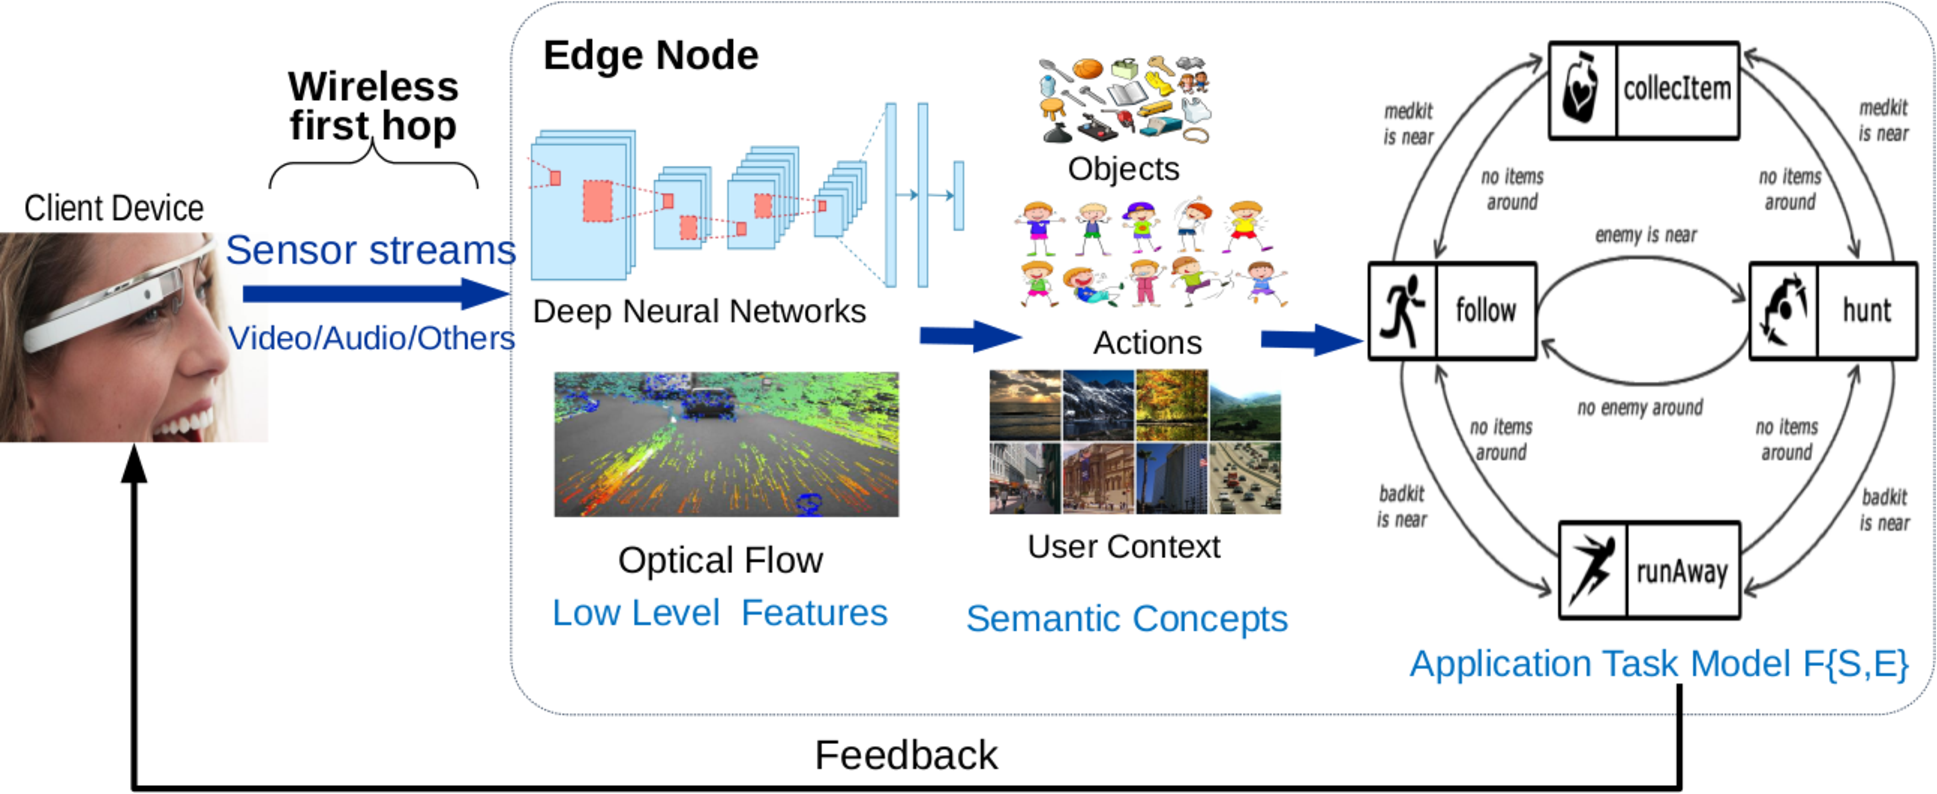
\includegraphics[width=.9\textwidth]{img/app_pipeline.pdf}
%         \captionof{figure}{Generic Human-in-the-loop Application Pipeline}
%         \label{fig:app-pipeline}
%     \end{minipage}%
% 	\begin{minipage}{.3\linewidth}
%     	\centering
% 		\includegraphics[width=\linewidth]{img/TraceReplay_GenArch}
%         \captionof{figure}{General architecture of the benchmarking suite.}
% 		\label{fig:TraceReplayArch}
% 	\end{minipage}
% \end{figure*}

% We furthermore argue that human-in-the-loop applications like AR potentially require costly gadgets for providing feedback to the human user. 
% Hence, this is another factor that contributes to the costs of such trials. 
% We hence strive for an approach to scalability tests of human-in-the-loop applications that can overcome these challenges while still sticking to an experimental approach in general.

%We address these challenges through an emulation approach.
%We address the discussed challenges on different levels.

To establish a reproducible and comparable workload, the first step in our methodology is to record a trace of the sensory input data while having a human user operate the target application. 
% The trace simply consists of the payload packets passed to the socket of the sensory device, which can be collected by TCP dump.
The collected data consists of the sensory inputs provided to the system at runtime, for instance, in the case of a visual application, the video feed from the camera.

To use the trace for reproducible experiments, we developed a benchmarking suite which can replay the trace to the original application, which results in the same computation to be performed on the edge as if a human was involved, while also ensuring a reproducible application execution path.
During the replay, many system level metrics can be collected, such as round-trip and processing times.
By enabling the client-side to play out the trace from a file, it becomes independent from human operation.
% For this, in particular a model of the human behavior needs to be defined and considered in the way the recorded trace is provided to the backend compute process. 

%\subsection{User Model}

In order to imitate a human behavior as close as possible, we propose the following user model as shown in Figure~\ref{fig:usermodel}.
We assume a user that is patient and does not make mistakes; any error message received from the application backend is ignored. We first divide a trace into steps that corresponds to individual events that should trigger feedback. If a positive feedback is received from the application, we jump ahead in the trace to replay the next step as if a human user reacts to the feedback. 
On the other hand, whenever the end of the current step is reached without having received any \emph{positive} feedback, the step is rewound a number $\tau$ of seconds.
To avoid infinite loops, where the application is stuck on a step forever, we have a maximum number of possible rewinds, after which the application shuts down.

\begin{figure}
    % Define block styles
    %         \tikzstyle{block} = [circle, draw, fill=red!20, 
    %         text width=5em, text centered, rounded corners, minimum size=4em]
    %         \tikzstyle{decision} = [diamond, aspect=2, draw, fill=yellow!20,
    %         text width=5em, text centered, rounded corners, minimum size=4em]
    %        \tikzstyle{line} = [draw, -{Latex[length=3mm]}]
    \centering
    \adjustbox{scale=0.75}{
        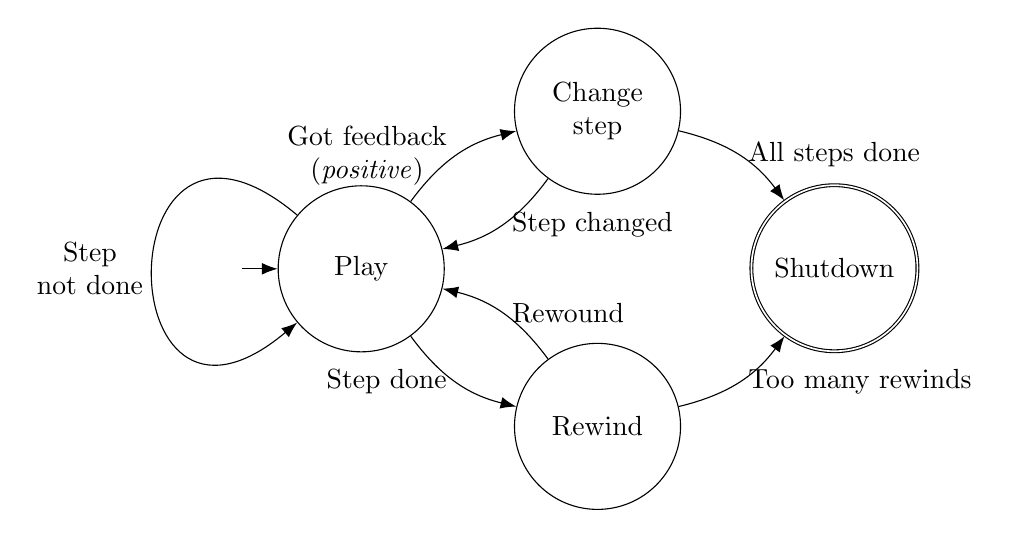
\begin{tikzpicture}[align=center,
        node distance=.5cm and 1.5cm,
        every initial by arrow/.style={-{Latex[length=2mm]}}]
        % Place nodes              
        \node [initial, state, minimum size=6em, initial text=] (play) {Play};               
        \node [state, above right=of play, minimum size=6em] (change) {Change\\step};
        \node [state, below right=of play, minimum size=6em] (rewind) {Rewind};
        \node [state, accepting, above right=of rewind, minimum size=6em] (shutdown) {Shutdown};
        
        
        
        % Draw edges
        \path[draw, -{Latex[length=2mm]}]
        (play) edge [bend right=20] node[left] {Step done} (rewind)
        edge [bend left=20] node[left] {Got feedback\\(\emph{positive})} (change)
        edge [out=140,in=220,looseness=6] node[left] {Step\\not done} (play)
        
        (change) edge [bend left=20] node[right] {Step changed} (play)
        edge [bend left=20] node[right] {All steps done} (shutdown)
        
        (rewind) edge [bend right=20] node[right] {Rewound} (play)
        edge [bend right=20] node[right] {Too many rewinds} (shutdown);
        
        \end{tikzpicture}
    }
    \caption{State diagram of the user model}
    \label{fig:usermodel}
\end{figure}

%A state diagram for the behavior of this user can be seen in Figure \ref{fig:usermodel}.

% Finally, by enabling this benchmark suite to run on commodity-of-the-shelf hardware, in our example we implemented the suite as an Android app, costs can furthermore be reduced by avoiding expensive gadgets to be available. 
% The suite is also based on a well-established cognitive assistance application framework, \emph{Gabriel} \cite{Chen:EarlyImplementation,Ha:TowardsWearableCogAssist}, which we believe will further aid in its adoption.

% In the following, we discuss the architecture and implementation of our benchmarking suite in more detail in particular with respect to wearable cognitive assistance applications.
% However, we stress that our methodology and in fact also our benchmark suite is applicable to most human-in-the-loop application as long as the backend code is available and the sensory input data can be captured.
% \footnote{We plan to make the benchmarking suite available to the community as Free and Open Source Software. Additionally, we plan to release the recorded traces under a Creative Commons License.}

\subsection{Architecture}

The suite has three elements, as shown in Figure~\ref{fig:TraceReplayArch}:
% the \emph{application backend}, the \emph{client emulator}, and the \emph{control backend} or \emph{server}, which interact in the following ways:

\begin{description}[labelindent=\parindent, listparindent=\parindent, style=unboxed, leftmargin=0cm]
  \item [The application backend] consists of instances of the target application running on Docker containers. 
  These correspond to real, unaltered instances of said cognitive assistance applications -- we do not model or emulate them in any way -- and they are containerized in order to be able to execute an arbitrary number of them on the same cloudlet.
  \item [The client emulator] consists of an Android application which emulates the behavior of a user operating the target cognitive assistance application while following the previously discussed user model.
  This Android app replays the previously recorded sensory data over the network to a specific \emph{application backend}, while collecting statistics and measurements of the system status. 
  %{\color{blue} Junjue: Should there be an application client in the picture? Logically, the benchmark android app feeds the application client the sensory information it needs, almost like hijacking the camera stream.}
  \item [The control backend] also runs on the cloudlet, although it could be executed in a separate cloud or cloudlet. It controls the execution of the experiments, by controlling the \emph{client emulators} over the network, initializing the \emph{application backends} and finally aggregating collected data when the experiments are completed. 
\end{description}

\begin{figure}
  \centering
  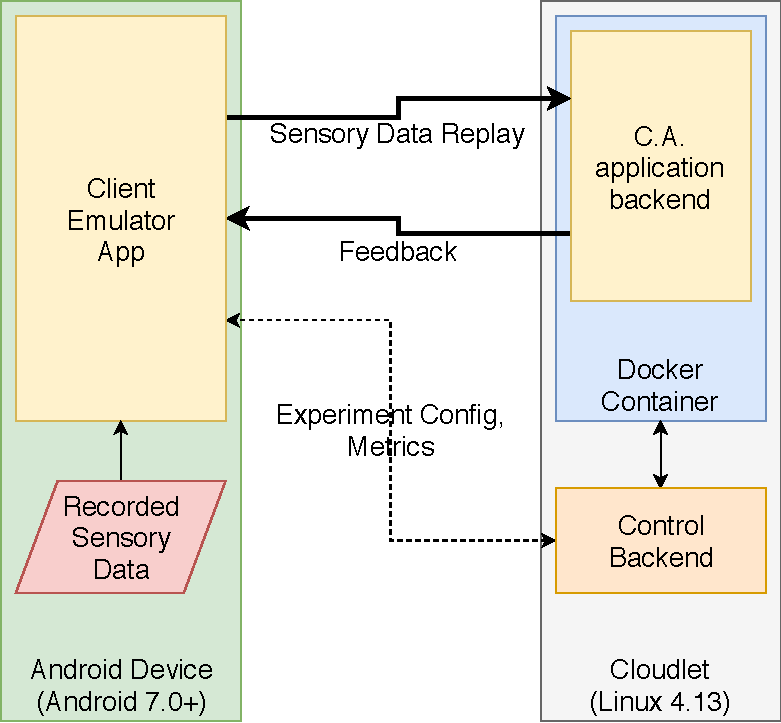
\includegraphics[width=.7\columnwidth]{publications/2018DemoScalingOnTheEdge/img/TraceReplay_GenArch}
  \captionof{figure}{General architecture of the benchmarking suite.}
  \label{fig:TraceReplayArch}
\end{figure}

\section{Demo Overview}

We will demonstrate the benchmarking framework using the \emph{LEGO Task Guidance} application previously developed by \textcite{Chen2015Early}.
This application guides a user step by step in the assembly of a LEGO model; input consists exclusively of video feed of the current state of the assembly, whereas feedback includes visual and auditory components in the form of animations and speech, respectively.

The benchmarking tool will be employed to extract key real-time metrics from this application, \emph{e.g.} average computation and network times, as well as the estimated \emph{user experience} level of the system as a whole (\emph{flawless}, \emph{impaired} or \emph{unusable}, based on the categorization in \cite{Chen2017Empirical}).

\section{Discussion and Future Work}

Some open questions and challenges remain to be tackled in the design and development of the presented tool.
To start with, the benchmarking suite is relatively narrow in the types of applications it can be applied to, currently only targeting event based cognitive assistance applications.
The tool needs to be extended to work on a much a broader spectrum of applications, in particular those that do not have a clear task model.
Furthermore, the current implementation does not support hardware accelerators (e.g. \acsp*{GPU}) that are commonly used for \ac{DNN} inference.

In addition, our current user model is simplistic. 
This model could be expanded to emulate a human user more accurately and realistically, e.g. making mistakes and responding to feedback to correct them.

We plan to extend our work in two directions. First, in addition to emulating user behaviors, we plan to simulate all the components in the system in order to generate reproducible experiments, test individual components of a real system, and identify performance bottlenecks when many users are using an application concurrently. Second, we are going to develop a statistical characterization of the application footprint, based on the data obtained from the tool.

\thesispaper{EdgeDroid}{Olguin:EdgeDroid2019}

\begin{abstract}
    %Benchmarking human-in-the-loop applications is complex.
%This limits reproducibility as well as feasibility of performance evaluations.
%In this paper we present EdgeDroid, a benchmarking suite that addresses these challenges.
%Our core idea rests on recording traces of these applications \jjw{-> application traces} which are then replayed out \jjw{remove out} in a controlled fashion based on an underlying model of human behavior \jjw{-> emulating human behaviors}.
%The traces are then exposed to the original backend compute process of the respective human-in-the-loop application, generating realistic feedback.
%This allows for an automated system that greatly simplifies benchmarking large scale scenarios.
%Our results confirm the utility of EdgeDroid as a tool for system designers, application developers and researchers.

%\jjw{Alternative version:
Many emerging mobile applications, including \acs{AR} and \acs{WCA}, aim to provide seamless user interaction.
However, the complexity of benchmarking these human-in-the-loop applications limits reproducibility and makes performance evaluation difficult.
In this paper, we present EdgeDroid, a benchmarking suite designed to reproducibly evaluate these applications.

Our core idea rests on recording traces of user interaction, which are then replayed at benchmarking time in a controlled fashion based on an underlying model of human behavior. 
This allows for an automated system that greatly simplifies benchmarking large scale scenarios and stress testing the application.
Our results show the benefits of EdgeDroid as a tool for both system designers and application developers.
%}

\end{abstract}
\section{Introduction}\label{paper:olguinmunoz2019edgedroid:sec:intro}

There is increasing interest from academia and industry in novel applications such as immersive \gls{AR} or \gls{WCA}~\cite{chatzopoulos2017hyperion,ha2014towards}, also known as human-in-the-loop applications.
These applications aim to seamlessly integrate into the lives of users to provide real-time, context-aware information by capturing user and environment information and leveraging compute-intensive algorithms to analyze the data in order to provide real-time feedback to the user.
Sensory input, such as video, audio, and other user-related data such as orientation and movement, are examples of what is typically captured, while the backend generally employs machine learning technologies such as \glspl{DNN}~\cite{ha2014towards}.
\Cref{paper:olguinmunoz2019edgedroid:fig:pipeline2} depicts such a system.
These applications are highly latency sensitive, measuring latency as the time from the capture of the sensory information until feedback is received.
Delays above a certain threshold can hurt the user experience or even make the application unusable~\cite{chen2017empirical}.

In literature, these challenging latency requirements have so far mainly been addressed through research on the optimal placement of the compute process.
There is a broad understanding today that with the advent of edge computing, human-in-the-loop applications will become viable~\cite{bittmann2017edge,flinn2012cyber,chen2017empirical,ha2013just}.
However, with respect to end-to-end latency, there are many more trade-offs involved than merely the question of where the compute backend is placed.
A human-in-the-loop application consists of various processing steps that can be influenced during the development of the application.
What kind of compression to apply to the sensory input on the uplink; which backend algorithms to utilize; how to stage the backend; when to send feedback to the human users; and how to manage congestion on the loop, as well as wireless channel fluctuations --- all these design choices impact the latency of the application.
There are also many design choices in the infrastructure: how is the sensory input conveyed to the point of computation (i.e.\ by which wireless system; with which transmission/prioritization scheme); which hardware is running at the backend; which operating system; how is the feedback conveyed back to the human user?
Finally, in production use these applications will most likely run concurrently with others.
How does this, together with other best-effort applications, impact the latencies perceived by the human user?
Existing studies~\cite{ha2014towards,chen2015early,satyanarayanan2009case,chatzopoulos2017hyperion} of this class of applications have only lightly touched upon these issues~\cite{chen2017empirical}.
On the other hand, recently published models for end-to-end latency of edge computing architectures~\cite{al_zubaidy2015performance,schiessl2017finite} are quite complex, while not accounting for the specifics of human-in-the-loop applications.
We only have a coarse understanding of the many degrees of freedom upon which end-to-end latency depends.

The goal of this paper is to provide a methodological approach to studying these latency trade-offs, along with a tool, EdgeDroid 1.0\footnote{We plan to make the EdgeDroid 1.0 benchmarking suite available as Free and Open Source Software and the recorded traces under a Creative Commons License.}, that simplifies the benchmarking of human-in-the-loop applications.
We view EdgeDroid 1.0 to be the very first, and simplest, of a family of tools that will embody increasingly sophisticated and accurate models of user behavior.

Due to the complex nature of the applications and the infrastructure, we opt for experimentally studying the trade-offs in a repeatable and controllable fashion.
This is difficult mainly due to the unpredictable reaction of human users to the feedback from the backend --- a user might very well misinterpret the feedback handed to them.
EdgeDroid 1.0 mimics the operation of human-in-the-loop applications by replaying recorded traces of sensory input.
This sensory information is then processed by the original compute process at the backend, generating feedback.
However, this feedback is not processed by humans, but by a parameterizable model of human reaction.
Through synchronized time tracking at the different processing points of the application, EdgeDroid 1.0 allows for accurate measurements of key performance metrics such as the distribution of delays across the application pipeline.
Analysis of these metrics can be performed down to the individual input sample, allowing us to zoom into the internal model of the application under consideration.
Thus, EdgeDroid 1.0 allows us to illuminate the many latency trade-offs existing at the level of the infrastructure, as well as the level of the application.
It can also be used for debugging and validation, by comparing the expected execution flow of a particular trace with the actual flow during the benchmarking.
To the best of our knowledge, this experimentally-driven benchmarking approach is the first one towards experimental performance characterization and potential optimization of human-in-the-loop applications

The rest of the paper is structured as follows:
\cref{paper:olguinmunoz2019edgedroid:sec:background} presents some background on human-in-the-loop applications.
\cref{paper:olguinmunoz2019edgedroid:sec:approach} discusses the general approach taken with EdgeDroid, while \cref{paper:olguinmunoz2019edgedroid:sec:implementation} exposes the implementation details for EdgeDroid 1.0.
We show the value of the tool through use case analysis in \Cref{paper:olguinmunoz2019edgedroid:sec:usecases,paper:olguinmunoz2019edgedroid:sec:results}, before discussing future work and concluding in \cref{paper:olguinmunoz2019edgedroid:sec:conclusions}.


%\section{Design \& Implementation}\label{sec:design_impl}
\section{Background}\label{paper:olguinmunoz2019edgedroid:sec:background}

Human-in-the-loop applications are novel applications aiming to seamlessly integrate into the lives of users and provide real-time, context-aware information.

Given the wide range of applications which fall under this concept, we have chosen to focus our initial efforts on one particular category: task-guidance \gls{WCA}~\cite{ha2014towards}.
We have chosen this type of application for two reasons: one, their relative simplicity in terms of execution flow, and two, the already well-established existing body of work~\cite{ha2014towards,chen2015early,chen2017empirical}.
Task-guidance \gls{WCA} applications aim to guide users in the execution of a task by monitoring user actions and providing real-time instructions, usually through wearable sensors and gadgets such as the Google Glass platform.
They have many potential use cases including training and assistance for professionals performing complex tasks.
Imagine for instance a specialized technician performing field repairs on a complex piece of machinery.
A task-guidance \gls{WCA} application could offer real-time guidance in this task, by analyzing a real-time video feed from the technician's head-mounted camera and providing step-by-step repair instructions.

Broadly speaking, task-guidance \gls{WCA} applications (and human-in-the-loop in general) process a multitude of inputs in parallel, which are also usually continuous, multidimensional and time-sensitive, e.g.\ video and audio feeds.
These inputs are passed to the computation backend, where they are processed in the pipeline depicted in \cref{paper:olguinmunoz2019edgedroid:fig:pipeline2}.
The first step of the backend processing is detection, which acts as a filter for irrelevant inputs.
For example, this step could consist of a computer vision detector which discards all frames for which the relevant features were not detected or which were below a set threshold.
%Given the often complex nature of the inputs, this stage usually employs Machine Learning to process them.
The remaining inputs pass on to the symbolic representation stage, where features are extracted and parameterized for subsequent computation.
For video frames, this parametrization would usually convert the visual data into a matrix representation of the  relevant features.
This representation of the inputs then continues on to the task model, where the actual application logic resides, before finally passing through the feedback generation stage at which point human-parseable feedback is generated; for instance, animations and voice commands.

\begin{figure}[b]
    \centering
    \adjustbox{scale=0.65}{
        \ttfamily\centering%\fbox{%
        \begin{tikzpicture}[align=center,
                        node distance=0.7cm and 0.7cm,
                        every initial by arrow/.style={draw=none, minimum size=0em},
                        %node styles:
                        block_center/.style ={rectangle, draw=black, thick, fill=white,
                                        text width=8em, text centered, minimum height=4em},
                        block_left/.style ={rectangle, draw=black, thick, fill=white,
                                        text width=16em, text ragged, minimum height=4em, inner sep=6pt},
                        block_noborder/.style ={rectangle, draw=none, thick, fill=none,
                                        text width=18em, text centered, minimum height=1em},
                        block_assign/.style ={rectangle, draw=black, thick, fill=white,
                                        text width=18em, text ragged, minimum height=3em, inner sep=6pt},
                        block_lost/.style ={rectangle, draw=black, thick, fill=white,
                                        text width=16em, text ragged, minimum height=3em, inner sep=6pt},
                        block_rounded/.style ={rectangle, draw=black, thick, fill=white,
                                        text width=8em, text centered, rounded corners=.55cm, minimum height=4em},
                        line/.style ={draw, thick, -{Latex[length=3mm]}, shorten >=0pt}
                ]

                \matrix [column sep=5mm,row sep=3mm] (top) {
                        \node [block_center] (detect) {Detection};
                         & \node [block_center] (repr) {Symbolic\\Repr.};
                         & \node [block_center] (model) {Task Model\\$M\{S, E\}$};
                         & \node [block_center] (feedback) {Feedback\\Generation}; \\[3ex]
                };

                \matrix [column sep=13mm,row sep=3mm, below=of top] (bottom) {
                        \node [block_rounded] (sensors) {On-body\\Sensors};
                         %& \node [block_rounded] (user) {Human User};
                         %&\node[cloud, draw, black, text centered, cloud ignores aspect=false] (user) {Human User};
                         & \node[maninblack, minimum height=5em] (user) {\Large Human User};
                         & \node [block_rounded] (hud) {HUD, Speakers,\\etc.}; \\
                };

                %\Smiley[1, below of=bottom] (smiley);


                \begin{scope}[every path/.style=line]
                        \path (detect) -- (repr);
                        \path (repr) -- (model);
                        \path (model) -- (feedback);
                        \path (feedback) -- (hud);
                        \path (hud) -- (user);
                        \path (user) -- (sensors);
                        \path (sensors) -- (detect);
                \end{scope}

                % % Place nodes       
                % \node [initial, state, draw=none, initial text=, minimum size=0em] (input) {};
                % \node [state, right=1cmof input, minimum size=7em] (detect) {Detection};
                % \node [state, right=2cm of detect, minimum size=7em] (symb) {Symbolic\\Repr.};
                % \node [state, right=.5cm of symb, minimum size=7em] (feedback) {Feedback\\Gen.};
                % \node [state, accepting, draw=none, right=1cm of feedback, minimum size=0em] (output1) {};
                % \node [state, accepting, draw=none, below=1.4cm of output1, minimum size=0em] (output2) {};

                % % Draw edges
                % \path[draw, -{Latex[length=3mm]}]
                % (input) edge node[above left] {Input} (detect)
                % (detect) edge node[above] {LEGO bricks\\in input} (symb)
                % (symb) edge node {} (feedback)
                % (feedback) edge node[above right] {Feedback} (output1)
                % (detect) edge [bend right=10] node[below left] {No LEGO bricks, thus no feedback} (output2) ;
        \end{tikzpicture}
}%}
    \caption{Pipeline of human-in-the-loop applications.}\label{paper:olguinmunoz2019edgedroid:fig:pipeline2}
\end{figure}

The task model of a task-guidance \gls{WCA} is a parameterized representation of the task in question and the steps required to complete it.
It can be represented as a Finite State Machine (FSM) \( M\{S, E\} \), where \(S\) is a set of states and \(E\) is a set of edges connecting these states.
Each state \(s_i \in S\) represents a configuration the application could potentially reach in an arbitrary execution, and each edge \(e_{i,j} \in E\) corresponds to the ability of the application to switch from state \(i\) to state \(j\) based on some user input.
We make a distinction between the set of \emph{steps} required to complete the task, \(S_s\), and \(S\), since the latter may also contain states which represent user mistakes in the execution of the task.
Thus, if we call the set of errors \(S_e\), we can further define \(S := S_s \cup S_e\).

\begin{figure}[tb]
    \centering
    \adjustbox{scale=0.75}{
    \ttfamily\centering%\fbox{%
    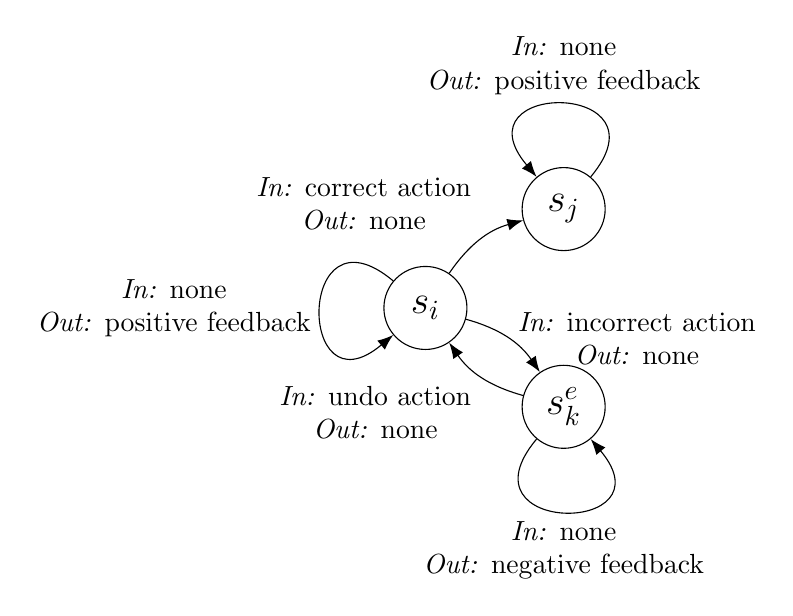
\begin{tikzpicture}[align=center,
        node distance=.5cm and 1cm,
        every initial by arrow/.style={-{Latex[length=2mm]}},
        line/.style ={draw, thick, -latex', shorten >=0pt}]
        % Place nodes       
        \node [state, minimum size=3em] (si) {\Large $s_{i}$};
        \node [state, above right=of si, minimum size=3em] (sj) {\Large $s_{j}$};
        \node [state, below right=of si, minimum size=3em] (se) {\Large $s^{e}_{k}$};

        \path[draw, -{Latex[length=2mm]}]
        (si)
        edge [out=140,in=220,looseness=6] node[left] {\emph{In:} none\\\emph{Out:} positive feedback} (si)
        edge [bend left=20] node[above left] {\emph{In:} correct action\\\emph{Out:} none} (sj)
        edge [bend left=20] node[right] {\emph{In:} incorrect action\\\emph{Out:} none} (se)

        (se)
        edge [bend left=20] node[below left] {\emph{In:} undo action\\\emph{Out:} none} (si)
        edge [out=230,in=310,looseness=6] node[below] {\emph{In:} none\\\emph{Out:} negative feedback} (se)

        (sj) edge [out=50,in=130,looseness=6] node[above] {\emph{In:} none\\\emph{Out:} positive feedback} (sj)
        ;

    \end{tikzpicture}
}%}
    \captionof{figure}{Segment of the internal task model of a linear task-guidance \acs{WCA}.}%
    \label{paper:olguinmunoz2019edgedroid:fig:taskmodel}
\end{figure}

These formalisms are exemplified in \cref{paper:olguinmunoz2019edgedroid:fig:taskmodel}, which represents an arbitrary segment of a linear task-guidance \gls{WCA} application.
\(s_{i}, s_{j} \in S\) represent sequential states in the execution of the task, with the edge \(e_{i,j}\) symbolizing the unique correct way of transitioning between them.
While in \(s_i\) and in the absence of inputs, the task model continuously provides instructions to the user on how to move to \(s_j\).
We will refer to this type of output as \emph{positive} feedback, since it guides the user forward in the execution of the task.
On the other hand, in the case of an erroneous input by the user, the task model moves to \(s^{e}_{k}\), where it will constantly provide instructions until the error is corrected and normal execution can resume.
This type of output directs the user to move backwards in the task model, and thus we will refer to it as \emph{negative} feedback.

\section{Approach of EdgeDroid}\label{paper:olguinmunoz2019edgedroid:sec:approach}

A system for benchmarking human-in-the-loop applications needs thus not only to be able to generate realistic, real-time inputs that follow the behavior of a real user but also be able to correctly react to feedback from the target application.
The design of EdgeDroid 1.0 tackles these challenges from two angles.
One, the generation of realistic inputs is delegated to a human user and provided to the suite in the form of a trace.
This ensures that the raw sensory input data is realistic.
Two, we propose the use of a \emph{user model} to adapt the replay of the trace to the task model and current system conditions.

Concretely, our proposed approach works in the following way:
\begin{enumerate}
    \item A trace of the sensory inputs for an execution of the task is recorded.
          For example, for a video-based application, this trace could consist of a recording from the point of view of a user performing the task.
          % Thanks to the user model, a single trace can be used for wildly different scenarios.
    \item This trace is \emph{manually} segmented into the logical steps which lead to the completion of the task.
          In other words for the generation of the trace the task model must be known to the human operator.
    \item The benchmarking suite is then configured to use this trace and a certain number of virtual users.
          This is done through a TOML~\cite{toml} configuration file on the backend.
    \item The benchmark is executed.
          Mobile devices are used to emulate users with wearable devices connecting to the \emph{real cloudlet} over the \emph{real network}.
          These devices replay the aforementioned trace, employing a \emph{user model} to adapt the trace to changing system conditions and navigate the task model to reach the desired system state.
          %\item The benchmarking suite finally outputs statistics and measurements once the benchmark finalizes.
\end{enumerate}

The extraction of metrics pertaining to the distribution of latencies across the application pipeline is the initial focus of EdgeDroid 1.0.
We calculate latencies by synchronizing clocks across the system components and storing timestamps at key points in the feedback loop.
These points include when input is sent and received, as well as when feedback is sent and received.
We collect raw data about each input-feedback cycle between user and cloudlet, which includes metrics on all the major steps in the feedback loop: uplink, downlink and processing time, presence of feedback, payload size, and so on.
This allows us to aggregate and obtain relevant statistics in postprocessing, such as average delays per step or distribution of average delays across the feedback loop.
We also store metadata regarding the task model with each measurement, for instance to link the state of the system with the current step being performed.

Note that this work does not directly target the \emph{motion-to-photon} latency metric.
This metric includes components such as sensing time and display time, which we do not consider.
We also do not evaluate the accuracy of the applications themselves, as we consider them to be \emph{black boxes}.
The system \emph{can} however be used to evaluate the trade-off between accuracy and performance, by comparing benchmarks performed using traces corresponding to different levels of accuracy.


\section{Implementation of EdgeDroid}\label{paper:olguinmunoz2019edgedroid:sec:implementation}

\begin{figure}[tb]
    \centering
    \includegraphics[width=.7\columnwidth]{publications/2019EdgeDroid/img/TraceReplay_GenArch}
    \caption{Architecture of the benchmarking suite.}\label{paper:olguinmunoz2019edgedroid:fig:TraceReplayArch}
\end{figure}

%In the following, we will detail the implementation of EdgeDroid 1.0.

The system architecture is composed of a \emph{cloudlet}, where one or more instances of the target application run, and one or more client devices, as pictured in \cref{paper:olguinmunoz2019edgedroid:fig:TraceReplayArch}.
These correspond to completely unaltered instances of the target application, running inside containers~\cite{docker}.
This allows the suite to extract metrics from them while remaining transparent to the application.
Here we also deploy the central component of EdgeDroid 1.0, the \emph{control backend}.

The \emph{control backend} is implemented in Python 3.6.
Its main purpose is to act as a central point of control and configuration of the experiments, as well as to aggregate results.
It controls the execution of the \emph{application instances} and configures the experiment and client devices, while also collecting system metrics during the execution of the benchmarks.
The experiments are configured in a centralized manner to simplify scaling.
Backend and clients communicate over TCP, using a simple application-layer protocol which allows for remote configuration, transmission of the trace data and result data, and synchronization of clocks across the system.
Note that although in the current implementation of the system the backend runs co-located with the \emph{application instances} on the cloudlet, we plan on implementing functionality for distributed monitoring from a separate computer and/or across multiple cloudlets.

The \emph{client emulators} correspond to Android applications with the main purpose of emulating a real user utilizing the target cognitive assistance application.
The emulators achieve this by mimicking the operation of real clients, but instead of obtaining the input data from the on-board sensors, they extract it from the previously recorded trace.
They replay this data over the network to the \emph{application instances} employing, as mentioned in \cref{paper:olguinmunoz2019edgedroid:sec:background}, a \emph{user model}, while simultaneously collecting client-side statistics and measurements.

The \emph{client emulators} are remote-controlled --- no interaction with a user is necessary once the application is initialized, simplifying large scale scenarios.

For our initial iteration of the EdgeDroid 1.0 benchmarking suite, we implement a preliminary user model, depicted in \cref{paper:olguinmunoz2019edgedroid:fig:usermodel}, to run on the \emph{client emulators}, designed with a linear task model in mind.
In EdgeDroid 1.0, our model is that of a user who is totally impervious to poor system performance, and suffers no annoyance, fatigue, frustration, nausea or other shortcomings of real human users.
This leads to a model of a user who responds in a precisely reproducible and deterministic manner to the same system stimulus every time.
In the future, we envision building upon this approach with many more human-like user models that more accurately emulate attributes such as fatigue and annoyance.

Each \emph{step} (i.e.\ segment) of the trace is played out to the backend until \emph{feedback} is received. If no feedback is received before the end of the step, it is replayed a pre-configured numbered of times before completely aborting the task (i.e.\ giving up).
Note that this model makes no distinction between positive and negative feedback, as both simply require the user to perform a specific action which is included in the trace.


\begin{figure}[tb]
    \centering
    \adjustbox{scale=0.7}{
    \ttfamily\centering%\fbox{%
    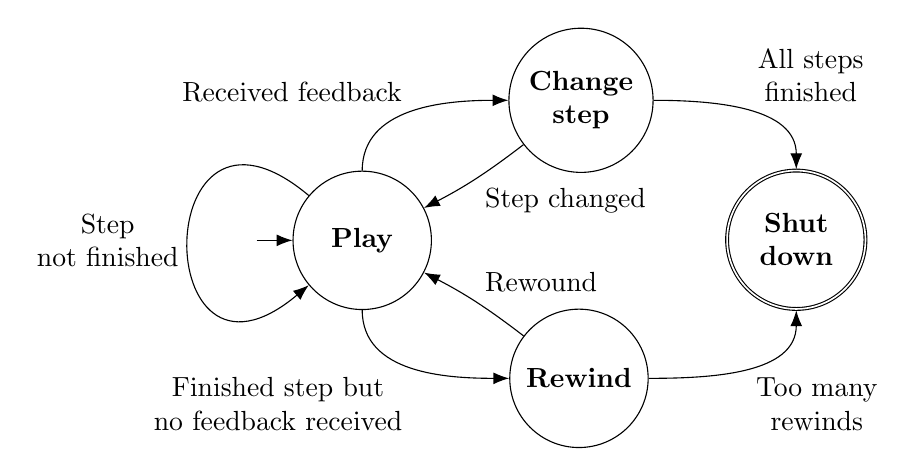
\begin{tikzpicture}[align=center,
        node distance=.5cm and 1.5cm,
        every initial by arrow/.style={-{Latex[length=2mm]}}]
        % Place nodes              
        \node [initial, state, minimum size=5em, initial text=] (play) {\textbf{Play}};
        \node [state, above right=of play, minimum size=5em] (change) {\textbf{Change}\\\textbf{step}};
        \node [state, below right=of play, minimum size=5em] (rewind) {\textbf{Rewind}};
        \node [state, accepting, above right=of rewind, minimum size=5em] (shutdown) {\textbf{Shut}\\\textbf{down}};

        % Draw edges
        \path[draw, -{Latex[length=2mm]}]
        (play) edge [out=270, in=180] node[below left] {Finished step but\\no feedback received} (rewind)
        edge [out=90, in=180] node[above left] {Received feedback} (change)
        edge [out=140, in=220,looseness=6] node[left] {Step\\not finished} (play)

        (change) edge [bend left=5] node[below right] {Step changed} (play)
        edge [out=0, in=90] node[above right] {All steps\\finished} (shutdown)

        (rewind) edge [bend right=5] node[above right] {Rewound} (play)
        edge [out=0, in=270] node[below right] {Too many\\rewinds} (shutdown);

    \end{tikzpicture}
}%}
    \captionof{figure}{Preliminary user model.}\label{paper:olguinmunoz2019edgedroid:fig:usermodel}
\end{figure}

\section{Use Cases}\label{paper:olguinmunoz2019edgedroid:sec:usecases}

\begin{table}[tb]
    \centering%
    \small%\ttfamily%
    \caption{Hardware used in the experiments.}%
    \label{paper:olguinmunoz2019edgedroid:tbl:cloudletclienthardware}%
    \begin{tabular}{@{}l@{\qquad}lclcl@{}}
        \toprule
         & \textbf{CPU}
         & \makecell{\textbf{Freq.}\\\textbf{[\si{\giga\hertz}]}}
         & \textbf{Cores}
         & \makecell[c]{\textbf{RAM}\\\textbf{[\si{\giga\byte}]}}
         & \makecell{\textbf{Operating}\\\textbf{System}}                                               \\
        \midrule
        \textbf{Cloudlet}
         & \makecell[bl]{Intel{\textregistered}\ Core{\texttrademark}\\i7--6700}
         & 3.4
         & 4
         & 32
         & \makecell[bl]{Ubuntu 17.10,\\kernel v4.13.0}                             \\
        \textbf{Clients}
         & \makecell[bl]{ARM{\textregistered}\\Cortex{\texttrademark}--A53}
         & 1.3
         & 4
         & 2
         & Android 7.0                                                             \\
        \bottomrule
    \end{tabular}%
\end{table}


In this section, we demonstrate the practical utility of EdgeDroid 1.0 through scalability measurements of real cognitive assistance application running on a cloudlet.
The questions we aim to answer relate to the ability of EdgeDroid 1.0 to provide relevant and accurate metrics on the performance of human-in-the-loop applications running on edge computing infrastructure.

Of particular interest is the ability to provide information about scaling limits in terms of latencies at both micro and macro levels.
We envision for instance a system designer performing the set of experiments detailed in this section.
The presented results would allow them to identify a bottleneck in performance.
From that they could extrapolate to how they need to scale their system hardware to manage their expected load, or they might conclude that their wireless link is not good enough for the average case.
They can also obtain real-time measurements to determine runtime measures to optimize performance, such as load balancing.
On the other hand, imagine an application developer who wishes to optimize their application.
EdgeDroid 1.0 would allow them to extract valuable information on where to focus their efforts.

%\todo[inline]{Also keep in mind that a perhaps more important question relates to on-line application optimization. Think about measures that can be applied at run-time on the side of the infrastructure to improve application performance - this is what one would like to explore here in this section.}

We chose the open source \emph{Gabriel} platform~\cite{ha2014towards} running the LEGO assistance application~\cite{chen2017empirical} for our experimentation.
This application guides a user through the assembly of a 2-dimensional LEGO model with visual and auditory instructions.
This functionality can be observed online.\footnote{\url{https://www.youtube.com/watch?v=7L9U-n29abg}}
We chose it due to its maturity and stability compared to other applications which run on the \emph{Gabriel} platform, as well as the relative simplicity of the task it performs.
The application employs a straightforward, linear task model as the one described in \cref{paper:olguinmunoz2019edgedroid:sec:background}.
Each state only allows for one specific correct action by the user, and any other action triggers negative feedback until the application is reset to the previous state.
The application has several different LEGO models to choose from, all of them roughly equal in complexity.
The specific task chosen for the experiments detailed in this section consists of the assembly of a 7-piece LEGO model.
The task has 7 distinct steps, and takes an average of approximately 2 minutes for a normal, untrained user to perform.
The input to the task model consist of a video stream captured either by an Android phone or a Google Glass wearable.

It should be noted that the \emph{Gabriel} platform by design always sends an acknowledgment for each input it receives, even when it is discarded, allowing us to measure latency for all inputs.


\cref{paper:olguinmunoz2019edgedroid:tbl:cloudletclienthardware} shows the hardware and software specifications for the cloudlet and the clients.
The components communicated through a single consumer-grade WiFi (IEEE 802.11n, \SI{2.4}{\giga\hertz}) access point.
We considered exclusively off-the-shelves hardware and software.
To minimize interference during the measurements, we locked the wireless link to the least congested available channel.
%Intel\textregistered \@ TurboBoost\texttrademark \@ technology was activated on the cloudlet CPU and the frequency of all cores locked to \SI{3.7}{\giga\hertz} to ensure consistency across experiments.

To ensure statistical independence between each emulated user, the initialization of each client emulator was subject to a random delay within a predefined window of time at the beginning of each run.
This way, the time between the start of any two clients in any repetition of the experiment is stochastic, leading to independent samples from each.
We also only take into account metrics collected while \emph{all} clients were concurrently running.

Our measurements were obtained from series of scenarios, repeated 100 times each.
We performed three \emph{optimal} scenarios with 1, 5 and 10 clients each, the signal strength of the WiFi link being an excellent \SI{-40}{\dBm}.
Next, a scenario where the 10 clients were moved to another room roughly \SI{10}{\meter} away, thus degrading the network link to an average measured strength of \SI{-73}{\dBm}.
Finally, we studied an additional optimal single-client scenario focused on latency distributions and jitters within application execution path.
This scenario is used to showcase the utility of EdgeDroid 1.0 for application developers.

\section{Results}\label{paper:olguinmunoz2019edgedroid:sec:results}

\begin{figure}
    \centering%
    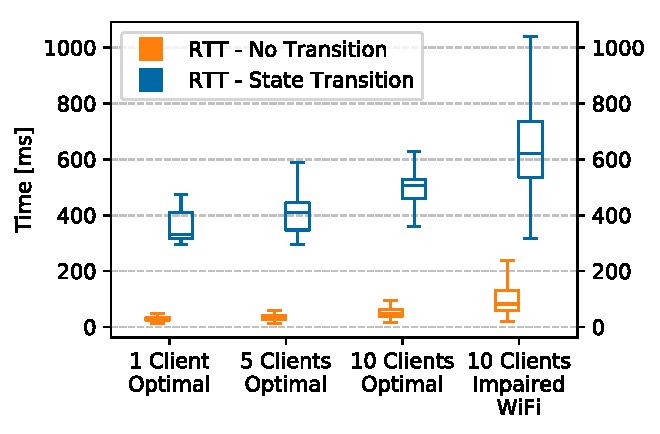
\includegraphics[width=.85\columnwidth]{publications/2019EdgeDroid/plots/comparison/nofonts/rtt_fb_vs_nofb}%
    \caption{Comparison of round-trip-times for inputs that triggered a state transition in the task model versus inputs that did not.}%
    \label{paper:olguinmunoz2019edgedroid:fig:comparison:rtt}%
\end{figure}%
\begin{figure}
    \centering%
    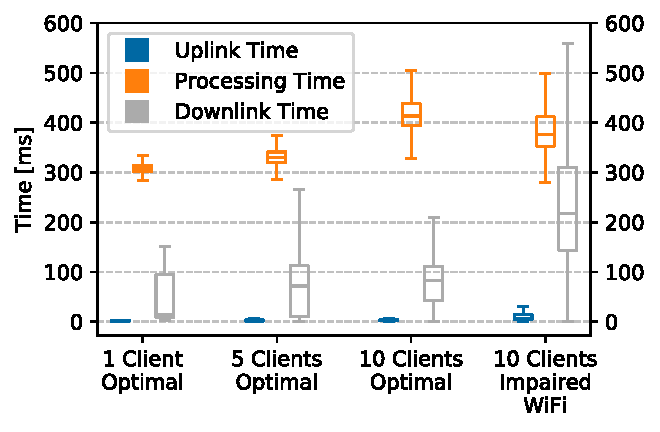
\includegraphics[width=.85\columnwidth]{publications/2019EdgeDroid/plots/comparison/nofonts/box_feedback}%
    \caption{Distribution of latency across system components for inputs that triggered a state transition in the task model.}%
    \label{paper:olguinmunoz2019edgedroid:fig:comparison:feedback}%
\end{figure}%
\begin{figure}%
    \centering%
    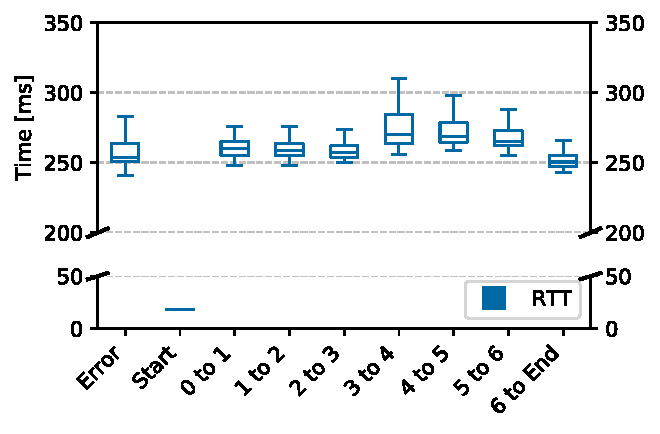
\includegraphics[width=.85\columnwidth]{publications/2019EdgeDroid/plots/comparison/nofonts/box_taskstep}%
    \caption{Round-trip-times for input-feedback cycles associated with state transitions in the internal task model for a single client connected over an optimal wireless link.}%
    \label{paper:olguinmunoz2019edgedroid:fig:comparison:tasksteps}
\end{figure}%

%In \cref{fig:comparison:feedback,fig:comparison:rtt,fig:comparison:tasksteps} we show some of the results obtained from the use case scenarios.
The results presented in this section provide valuable insights on both the system limits as well as on the application itself.

\cref{paper:olguinmunoz2019edgedroid:fig:comparison:rtt} presents a comparison of the total measured round-trip-times (RTTs) both for inputs which caused a state transition and inputs that did not.
Next, \cref{paper:olguinmunoz2019edgedroid:fig:comparison:feedback} shows a comparison of the distribution of latencies across system components for inputs that caused an internal state change in the task model of the application.
We differentiate according to the three main components contributing to latency, namely \emph{uplink} and \emph{downlink transmissions}, and \emph{backend processing}.
Finally, \cref{paper:olguinmunoz2019edgedroid:fig:comparison:tasksteps} depicts the distribution of RTTs for each transition in the internal task model for a single client connected over an optimal wireless link.
These metrics were calculated by recording the measured input-feedback cycle delay corresponding to a change in state within the application.
Thus, for instance, the measurements located at column ``3 to 4'' in the figure correspond to the aggregated round-trip-times for every input-feedback cycle corresponding to a change from state 3 to state 4 within the application task model, for the 100 repetitions of the scenario.

In the following discussion we will refer to inputs which triggered a transition in the task model as \emph{feedback-rich inputs} and those that did not as \emph{feedback-less inputs}.

For the analysis of these results, we will take into consideration the bound of \SI{600}{\milli\second} response time for step-by-step task-guidance derived by the authors of~\cite{chen2017empirical}.
This bound marks the point after which further delays in the delivery of feedback to the user start to negatively affect user experience, and allows for a straightforward evaluation of the responsiveness of the system.

We will begin our analysis of the experiment results with \cref{paper:olguinmunoz2019edgedroid:fig:comparison:rtt}.
These results present a stark contrast in the round-trip-times for inputs which cause a state transition versus inputs that do not, with RTTs for the former being up to an order of magnitude greater.
It's worth mentioning though that responses to feedback-less inputs are invisible to the user, and are just included here as a sort of baseline to compare feedback-rich round-trip times with.

We can identify a pair of interesting effects in the scaling of the task-guidance \gls{WCA} application.
One, scaling behavior for the application seems to be linear with respect to the number of clients.
Two, in the case of the impaired WiFi, the effect on the feedback-rich inputs is very pronounced, with the average of the RTTs for these inputs being over the previously discussed bound of \SI{600}{\milli\second}.

It is worth noting that already at just 10 clients the response times for feedback-rich inputs are very close to the bound.
Looking at this through the lens of a an application developer, it could hint at a need for optimization of the later parts of the application pipeline, since RTTs for inputs which are discarded in the detection stage of the pipeline (i.e.\ feedback-less inputs) are still well below \SI{200}{\milli\second}.

EdgeDroid 1.0 allows researchers to zoom into specific components of the application feedback loop, as exemplified by \cref{paper:olguinmunoz2019edgedroid:fig:comparison:feedback}.
From this figure it is clear that the main component which contributes to latency in the optimal case is the backend processing, further lending credibility to our previous comment on the need for optimization.
Nevertheless, when the link quality decreases, the delays on the downlink start to overshadow the delays on the processing.
Here, the downlink time sometimes almost reaches the ideal bound by itself.
A system designer might then conclude from this that in order to be able to scale the application, their focus needs to be on improving the quality of the wireless link before increasing the processing power on the backend.

Finally, EdgeDroid 1.0 allows even more insights to be gained by homing in to individual steps in a task-guidance \gls{WCA}. Consider \cref{paper:olguinmunoz2019edgedroid:fig:comparison:tasksteps}.
The figure shows clears spikes in latencies at the transitions from task state 3 to 4 and from task state 4 to 5, which could indicate to the application developer that these specific transitions are ripe for optimization.

\section{Conclusions \& Future Work}\label{paper:olguinmunoz2019edgedroid:sec:conclusions}

Benchmarking human-in-the-loop applications is hard, given their tight interaction with human users who complicate the scaling and repeatability of experiments.
In this paper, we have presented a benchmarking suite for this type of applications, called EdgeDroid 1.0, capable of cutting out the need for users in performance evaluations.
We achieve this by employing pre-recorded sensory input traces which we play over the network to the real application backend, employing a parameterized user model to react to feedback.
We demonstrate its utility through a series of use case scenarios, from which we are able to extract metrics regarding latency both in regards to the application itself and the hardware stack.
We believe the EdgeDroid 1.0 suite thus represents an important first step towards enabling inexpensive and low-complexity large-scale research on the scaling limits of this type of applications, a requirement for wide adoption of the technology.

Nonetheless, there is still future work to be done.

The user model presented in this paper is only preliminary, and we are currently conducting research in characterizing user behavior when interacting with \gls{WCA} applications in order to present a more complete model in the future.
As mentioned in \cref{paper:olguinmunoz2019edgedroid:sec:implementation}, in EdgeDroid 1.0, our model is that of a user who does not suffer any of the shortcomings of real human users such as annoyance, fatigue, frustration, nausea.
Rather, EdgeDroid 1.0 models a perfectly stoic user who is like an automaton and responds in a precisely reproducible and deterministic manner to the same system stimulus every time.
Of course, no real human user is an automaton.
In the future, we envision creating  many versions of EdgeDroid (i.e., EdgeDroid 2.0, EdgeDroid 3.0, etc.) that embody more human-like user models that more accurately emulate attributes such as those mentioned above.
Experimental validation of these human-like user models via user studies will be an important part of our future work.

We are also working on expanding the benchmarking suite to also work first with other types of Wearable Cognitive Assistance, and later with other categories of human-in-the-loop applications.
Other types of \glspl{WCA} we will consider in future iterations of the tool include real-time task-assistance \gls{WCA} applications (such as the Ping-Pong application described in~\cite{chen2017empirical}), which don't have a linear task model like task-guidance \gls{WCA} and have tighter latency bounds and context- and information-providing \gls{WCA} applications, for instance, applications which recognize faces and provide relevant social-media information related to that person.
The latter also do not have a linear task model, but present more lax latency bounds.

\begin{acks}
    We thank Bobby Klatzky and Dan Siewiorek for many valuable technical discussions relating to this research.
    We also thank our shepherd, Wenjun Hu, and the anonymous reviewers for helping us improve the paper.
    This research was supported in part by the \gls{NSF}, grant number \verb|CNS-1518865|, the VINNOVA grant \verb|MERIT (2017--05232)|.
    Additional support was provided by Intel,\ Vodafone,\ Deutsche~Telekom,\ Verizon,\ Crown~Castle,\ NTT,\ and the Conklin~Kistler family fund.
    Opinions, findings, conclusions or recommendations expressed in this material are those of the authors and do not necessarily reflect the view(s) of their employers or the mentioned funding sources.
\end{acks}

\end{appendices}

\end{document}
\endinput
%%
%% End of file `kth-demo.tex'.
